\documentclass[twoside,twocolumn]{mnras}

% Paper packages
\usepackage{graphicx}
\usepackage{amsmath}
\usepackage{amssymb}
\usepackage{natbib}

% Define astronomical units
\newcommand{\msun}{\ensuremath{M_{\odot}}}
\newcommand{\pc}{\ensuremath{\rm pc}}
\newcommand{\kms}{\ensuremath{\rm km\,s^{-1}}}

\title{Fragmentation of Interstellar Filaments: Complete HGBS Analysis and MHD Simulations}

\author[G.~J.~White]{G.~J.~White$^{1,2}$\\
$^{1}$School of Physical Sciences, The Open University, Walton Hall, Milton Keynes, MK7 6AA, UK\\
$^{2}$Rutherford Appleton Laboratory, Harwell Science and Innovation Campus, Didcot, OX11 0QX, UK}

\begin{document}

\maketitle

\begin{abstract}
Classical fragmentation theory predicts core spacing ${\sim}4\times$ the filament
width, yet Herschel measures $\lambda/W \approx 2$--$3$. We reanalyse core spacing
in Herschel Gould Belt Survey (HGBS) filaments using Gaia DR3 distances and 2,013
self-gravitating MHD simulations.

\textbf{Primary limitations}: (1) \textit{Perpendicular-field paradox}: Planck~(2016) shows ${\sim}90\%$ of dense filaments have magnetic fields perpendicular to their axes, yet our perpendicular-field simulations give $\lambda/W_{\rm fil} \approx 0.76$--$0.88$---a factor ${\sim}3\times$ below the observed $2.79$. \textbf{If this paradox is unresolved, single-component MHD fragmentation cannot explain the dominant filament population.} (2) \textit{Supercritical extrapolation}: All 654 supercritical simulations ($f \geq 1.5$) yield pure radial collapse; \textit{the simulations cannot directly measure $\lambda/W$ for 30--50\% of actively star-forming filaments}. All simulation--observation comparisons rest on near-critical ($f = 0.9$--$1.3$) calibration only.

Observationally, the full 8-region sample (5,069 cores) gives $\lambda/W = 2.79 \pm 0.025$~pc (pairwise median; four robust regions give $2.84 \pm 0.026$~pc). After 3D projection correction the inferred spacing is ${\sim}3.5\times W$, within 15\% of the classical prediction \citep{Inutsuka1992}. Magnetic tension for longitudinal fields ($\beta \leq 0.5$) is viable at $\eta_W \approx 0.606$ but excluded at $\eta_W \approx 0.707$; the 17\% $\eta_W$ uncertainty currently prevents assessment of this scenario. Hierarchical fibre fragmentation (sub-filaments with longitudinal fields below Planck resolution) is observationally suggested by single-region data \citep{Yang2024} but is untested by our simulations.

Simulations reveal $1/t_{\rm frag} \propto f^{0.39}$ ($r^2 = 0.999$). Near-critical filaments ($f \lesssim 1.2$) produce longitudinal beading. The $\eta_W$ uncertainty dominates all other theoretical uncertainties; independent validation is required before magnetic tension can be assessed.
\end{abstract}

\begin{keywords}
stars: formation -- ISM: structure -- ISM: filaments -- MHD -- turbulence
\end{keywords}

\section{INTRODUCTION}

The \textit{Herschel} Space Observatory established that filaments are the fundamental
structures within which star formation occurs in molecular clouds \citep{Andre2010}.
Two key observational results emerged: (1) a characteristic filament width of $\sim$0.1~pc
across diverse environments \citep{Arzoumanian2011}, and (2) a critical mass-per-unit-length
of $M_{\rm line,crit} \approx 16~M_\odot$/pc \citep{Ostriker1964}.

Classical fragmentation theory \citep{Inutsuka1992} predicts that isothermal gas cylinders
fragment at a wavelength of approximately $4\times$ the filament width. For the
characteristic HGBS width of $0.10$~pc, this predicts a core spacing of $\sim 0.4$~pc.
Original HGBS analyses measured spacings of $\sim 0.2$~pc---nearly a factor of two below
this prediction. With Gaia DR3 distances \citep{Zhang2023}, measured spacings have
increased to $\sim 0.28$~pc, reducing the discrepancy to a factor of 1.4.

Two primary explanations have been proposed. First, \textbf{hierarchical fragmentation}:
high-resolution studies show that filaments consist of velocity-coherent fibres
\citep{Hacar2013}, and recent work in Orion~B \citep{Yang2024} shows that fibre-to-core
spacing recovers the classical $4\times$ prediction while filament-to-core measurements
show sub-Jeans values. Second, \textbf{magnetic tension}: longitudinal fields shift the
most unstable mode to shorter wavelengths \citep{Nakamura1993}, predicting
$\lambda/W \approx 2.44$--$3.16$ for equipartition fields ($\beta \sim 1$--$3$).

\textbf{A fundamental challenge}: Planck~(2016) established that ${\sim}90\%$ of dense HGBS filaments have magnetic fields perpendicular to their long axes. Our perpendicular-field simulations give $\lambda/W_{\rm fil} \approx 0.76$--$0.88$---a factor ${\sim}3\times$ below the observed $2.79$. This creates a severe paradox: \textbf{if the Planck field geometry applies to filament interiors (not just envelopes), then single-component MHD fragmentation cannot explain the dominant filament population.} This paper explicitly foregrounds this paradox; we test three possible resolutions in Section~\ref{sec:perp_paradox}, but none are currently confirmed by observations or simulations. Resolving this paradox requires interior polarimetric mapping at sub-Planck resolution.

Here we present a systematic analysis of all 8 high-confidence HGBS regions using Gaia DR3 distances and a uniform pairwise-median methodology, combined with 2,013 self-gravitating MHD simulations. Observationally, hierarchical fibre fragmentation is suggested by single-region data from \citealt{Yang2024} (Orion~B only) but remains observationally unconfirmed in other HGBS regions; \textbf{none of the 2,013 simulations model multi-fibre fragmentation}, and the simulations constrain only single-component MHD fragmentation. All 654 supercritical ($f \geq 1.5$) simulations yield pure radial collapse; the simulation--observation comparison rests on near-critical ($f = 0.9$--$1.3$) calibration only. Magnetic tension in a strictly longitudinal, low-$\beta$ geometry is a secondary possibility, viable at $\eta_W \approx 0.606$ but excluded at $\eta_W \approx 0.707$ (Section~\ref{sec:width_correction}).

\section{OBSERVATIONAL ANALYSIS}

\subsection{Complete HGBS Sample}
\label{sec:sample}

Our sample includes 8 high-confidence HGBS regions (Table~\ref{tab:sample}), with
distances updated to Gaia DR3-based measurements from \citet{Zhang2023}.

\textbf{Distance revisions}: The most significantly affected regions are Serpens
($260 \to 458$~pc, $+76\%$), Aquila ($260 \to 436$~pc, $+68\%$), and Orion~B
($260 \to 386$~pc, $+48\%$). Taurus shows a small decrease ($140 \to 135$~pc, $-4\%$).

\textbf{Core selection}: We include starless, prestellar, and protostellar cores following the standard HGBS framework \citep{Konyves2015, Konyves2020}. As a cross-check, using only the 331 Taurus starless cores gives $\lambda/W = 2.03$---within 2.5\% of the all-core value---confirming that protostellar inclusion does not bias the result.

\begin{table*}
\caption{Complete HGBS Sample with Gaia DR3 Distances}
\label{tab:sample}
\begin{tabular}{lcccccc}
\toprule
Region & Distance & Total & Spacing & Std Error & Beam (pc) & Status \\
       & (pc)   & Cores & (pc)   & (pc)      & (pc) & \\
\midrule
Orion B  & 386 & 1,844 & 0.313 & 0.047 & 0.034 & Robust \\
Aquila   & 436 & 749   & 0.346 & 0.047 & 0.038 & Robust \\
Perseus  & 296 & 816   & 0.248 & 0.040 & 0.026 & Robust \\
Taurus   & 135 & 536   & 0.198 & 0.040 & 0.012 & Robust \\
Ophiuchus& 137 & 513   & 0.206 & 0.053 & 0.012 & Limited \\
Serpens  & 458 & 194   & 0.331 & 0.097 & 0.040 & Limited \\
TMC1     & 135 & 178   & 0.195 & 0.056 & 0.012 & Limited \\
CRA      & 150 & 239   & 0.248 & 0.072 & 0.013 & Limited \\
\midrule
\textbf{Weighted Mean} &  & \textbf{5,069} & \textbf{0.279} & \textbf{0.009} & --- &  \\
\bottomrule
\end{tabular}
\\ \footnotesize \textbf{Note}: Beam scale = 18$''$ FWHM. Ophiuchus is classified as Limited (not Robust) despite $N>500$ because of larger distance uncertainty and slightly lower completeness.
\end{table*}

\subsection{Measurement Methodology}

Filament skeletons were identified using DisPerSE \citep{Sousbie2011} following standard
HGBS methodology with a $3\sigma$ persistence threshold and a robustness/filament-contrast
threshold of $\kappa = 2.0$ (standard HGBS parameters; \citealt{Arzoumanian2011}). Gaia DR3 distance revisions
do not require re-extraction of skeletons; physical scales are updated by rescaling
angular positions. Core-to-core spacings were measured using the pairwise median
statistic: for a filament with $N$ cores, we compute all $N(N-1)/2$ pairwise distances
and take the median. Cores were associated with filaments using a perpendicular
distance threshold of $2\times$ the characteristic filament width; results change
by $<3\%$ across threshold choices of $1$--$2\times W$.

\subsection{Results}
\label{sec:results}

\textbf{Width systematic}: A $\sim$30\% systematic uncertainty from filament width
scatter ($0.05$--$0.20$~pc; \citealt{Panopoulou2022}) affects all $\lambda/W$ values
and is not included in bootstrap error bars; it dominates when comparing with theory.

\textbf{Primary result}: Four robust regions (Orion~B, Aquila, Perseus, Taurus;
$N > 500$) give $0.284 \pm 0.026$~pc jackknife ($\lambda/W = 2.84$; bootstrap
$\pm 0.012$~pc); the full 8-region sample gives $0.279 \pm 0.025$~pc jackknife
($\lambda/W = 2.79$; bootstrap $\pm 0.009$~pc). Jackknife errors are adopted as
primary throughout (Section~\ref{sec:statistics}); bootstrap CI given for reference.
Gaia DR3 raised the mean 32\% from $0.211$~pc; leave-one-out analysis
(Table~\ref{tab:leave_one_out}) shows no single region dominates ($\Delta < 6\%$);
leave-two-out (Aquila+Orion~B excluded) gives $0.231$~pc ($\lambda/W = 2.31$,
$\Delta = -16.8\%$; Table~\ref{tab:leave_one_out}).

Figure~\ref{fig:spacing} shows the spacing measurements. After the standard 3D projection
correction, we adopt $4/\pi \approx 1.27$ \citep{Andre2010}, corresponding to the
\citet{Hacar2013} finite-aspect-ratio value for filaments with aspect ratios ${\sim}10{:}1$
(range 1.18--1.41 for $5{:}1$--$20{:}1$; we adopt the fiducial $10{:}1$ value, systematic
uncertainty $\lesssim 10\%$). The inferred spacing is ${\sim}3.5\times W$, within 15\%
of the classical $4\times$ prediction.

\textbf{Planck-informed projection}: \citet{Planck2016} find that dense filaments lie
preferentially in the plane of sky (B-field perpendicular to filament axis, B
predominantly in sky plane). Under this geometry the projection factor reduces from
$4/\pi \approx 1.27$ to ${\sim}1.10$--$1.20$, giving a corrected spacing of only
${\sim}3.1$--$3.3\times W$---\textit{strengthening} the residual discrepancy with the
$4\times$ prediction \citep{Inutsuka1992} rather than resolving it. The headline claim
of ``within 15\% of the classical prediction'' applies to the random-orientation
correction; under the Planck-motivated geometry the discrepancy is $18$--$22\%$.
We adopt $4/\pi$ for literature comparability; the Planck-informed correction
represents an important additional caveat.

\begin{table}[h]
\caption{Leave-One-Out Sensitivity Analysis}
\label{tab:leave_one_out}
\begin{tabular}{lcccc}
\toprule
Excluded Region & Excl.\ spacing (pc) & Remaining mean (pc) & $\lambda/W$ & $\Delta$ (\%) \\
\midrule
None (full sample) & --- & 0.279 & 2.79 & 0.0 \\
Orion B & $0.313 \pm 0.047$ & 0.268 & 2.68 & $-3.9$ \\
Aquila & $0.346 \pm 0.047$ & 0.266 & 2.66 & $-4.7$ \\
Perseus & $0.248 \pm 0.040$ & 0.281 & 2.81 & $+0.7$ \\
Taurus & $0.198 \pm 0.040$ & 0.287 & 2.87 & $+2.9$ \\
Ophiuchus & $0.206 \pm 0.053$ & 0.286 & 2.86 & $+2.5$ \\
Serpens & $0.331 \pm 0.097$ & 0.276 & 2.76 & $-1.1$ \\
TMC1 & $0.195 \pm 0.056$ & 0.281 & 2.81 & $+0.7$ \\
CRA & $0.248 \pm 0.072$ & 0.279 & 2.79 & $0.0$ \\
\midrule
Robust only & --- & 0.284 & 2.84 & $+1.8$ \\
\textbf{Aquila $+$ Orion~B excl.} & --- & \textbf{0.231} & \textbf{2.31} & $\mathbf{-16.8}$ \\
\bottomrule
\end{tabular}
\vspace{2pt}
\footnotesize Bootstrap 95\% CI $[0.261, 0.298]$~pc; jackknife $1\sigma$: full sample $\pm 0.025$~pc; robust $\pm 0.026$~pc. With $N=8$ regions the bootstrap spans only $2^8=256$ distinct resamples, making the jackknife more reliable at this sample size. Excluding the two highest-revision regions (Aquila $+68\%$, Orion~B $+48\%$) reduces the mean by $16.8\%$; their Gaia distances are independently confirmed \citep{Yan2022,Green2024,Kounkel2018}, so this sensitivity reflects the real importance of accurate distances rather than systematic bias.
\end{table}

\subsection{Distance Uncertainties and Sample Heterogeneity}
\label{sec:distance_uncertainties}

We classify regions as \textbf{Robust} (Orion~B, Aquila, Perseus, Taurus: $N>500$,
well-established Gaia distances, $<15\%$ or validated revision) or \textbf{Limited}
(Ophiuchus, Serpens, TMC1, CRA (Corona Australis): smaller YSO samples and/or $>50\%$ revision).

\textbf{Serpens}: The +76\% distance revision ($260 \to 458$~pc) raises concern, but is independently confirmed at $440$--$460$~pc \citep{Yan2022, Green2024, Zucker2020}. Excluding Serpens changes the full-sample result by only 1.1\% (Table~\ref{tab:leave_one_out}).

\textbf{Serpens beam/completeness}: The $0.040$~pc beam (40\% of $W_{\rm fil}$) may
overestimate spacing by ${\sim}8\%$; at 3.8\% sample weight, impact on the mean is
$<0.2\%$. Serpens is classified as Limited.

\textbf{Aquila anomaly}: Aquila has the largest Robust spacing ($\lambda/W = 3.46$),
elevated by the $+68\%$ distance revision and possibly W40 H\,{\sc ii} feedback.
The W40 ionisation front has swept material to radius ${\sim}1$~pc; the
photodissociation region (PDR) extends ${\sim}2$--$3$~pc \citep{Bontemps2010,
Strafella2015}. The Aquila filament network spans ${\sim}4$~pc; cores in the feedback
zone may have systematically wider spacings due to turbulent injection, constituting an
unresolved environmental contamination. The 436~pc distance is confirmed by 3D dust
mapping \citep{Zucker2020} and Gaia-parallax YSOs at $430 \pm 20$~pc
\citep{Konyves2020}. Aquila is retained as Robust but flagged as an environmental outlier;
exclusion reduces the robust mean by 6\%.

\textbf{Aquila protostellar cross-check}: Monte Carlo resampling retaining 663 non-protostellar sources gives $\lambda/W = 3.40 \pm 0.07$ vs.\ all-core value 3.46 ($<2\%$ change); this demonstrates pairwise-median robustness to core-type contamination, not absence of protostellar migration effects.

\textbf{Distance-spacing regression}: As expected, $\lambda \propto d$ ($r^2 = 0.91$;
the relationship is geometric, not evidence for physical uniformity). The residuals
test ($r = 0.18$, $p = 0.68$) demonstrates no obvious systematic bias in the
distance revisions, but with $N = 8$ regions this test has low statistical power
(type~II error rate ${\sim}60\%$) and cannot provide strong evidence against
systematic bias.

\subsection{Statistical Methods: Pairwise Median and Uncertainties}
\label{sec:statistics}

\textbf{L/3 convergence bias --- bounding analysis}: For a uniform distribution of
$N$ cores on a filament of length $L$, the pairwise median converges toward
$(1-1/\sqrt{2})L \approx 0.293L$ (denoted $L/3$ hereafter).

\textit{Clustering-scale argument}: If L/3 dominated, regional pairwise medians
should scale as $\lambda_{\rm PM} \approx 0.293L$ and vary in proportion to filament
length. For $L \approx 0.5$--$3$~pc \citep{Arzoumanian2019}, this predicts a factor
$6\times$ spread in measurements. Our 8-region values span $0.198$--$0.346$~pc (factor
$1.75\times$), inconsistent with L/3 dominating across regions with such varied lengths.
The tight clustering of measurements near $0.28$~pc implies a physical scale.

\textit{Uniform-null exceedance}: For individual filaments with $L \lesssim 0.68$~pc,
the uniform-null ($0.293L \leq 0.20$~pc) falls at or below our minimum measurement.
For these short filaments, our measurement \textit{exceeds} the purely uniform
prediction, providing direct evidence against L/3 domination. For longer filaments
($L \sim 2$--$3$~pc), this test is inconclusive.

\textit{Taurus nearest-neighbour check}: $\lambda_{\rm NN} = 0.217 \pm 0.052$~pc
vs.\ $\lambda_{\rm PM} = 0.198$~pc. The pairwise median is \textit{lower} than the
nearest-neighbour spacing---qualitatively opposite to L/3 inflation.

\textbf{Conclusion}: The L/3 bias is unquantified for 7 of 8 regions (raw positional
data required). The clustering-scale and null-exceedance arguments suggest the bias is
not dominant, but neither constitutes a rigorous proof. \textbf{It remains the
dominant systematic uncertainty.}

\textbf{Jackknife vs.\ bootstrap}: With $N = 8$ regions the bootstrap spans only
$2^8 = 256$ distinct resamples; the jackknife standard error ($\pm 0.025$~pc full;
$\pm 0.026$~pc robust) is more reliable. Bootstrap 95\% CI $[0.261, 0.298]$~pc is
given for reference.

\textbf{Bayesian hierarchical model}: Treating the 8 regional measurements as draws
$\lambda_i | \mu, \sigma_{\rm pop} \sim \mathcal{N}(\mu, \sigma_{\rm pop}^2)$ with
uniform priors yields: $\sigma_{\rm pop} = 0.062$~pc (genuine region-to-region
scatter), posterior $\mu = 0.261 \pm 0.022$~pc (68\% CI), 95\% CI $[0.217, 0.305]$~pc.
The $N$-weighted mean ($0.279$~pc) is elevated by the core-rich Orion~B and Aquila
regions; the Bayesian unweighted mean is $6\%$ lower but consistent within
$1\sigma_{\rm pop}$. The $\sigma_{\rm pop} = 0.062$~pc scatter is genuine
region-to-region heterogeneity, not measurement noise; it is the dominant uncertainty
on the population mean.

\textbf{HGBS window}: The observational window $[2.52, 3.08]$ represents
$2.79 \times [0.90, 1.10]$---a $\pm 10\%$ band matching the dominant $10\%$ uncertainty
on $W = 0.1$~pc \citep{Panopoulou2022}; the jackknife measurement uncertainty ($\pm 9\%$)
is comparable. The window thus corresponds to $1\sigma$ of the width systematic.


\subsection{Comparison with Literature}

Our Gaia DR3 measurements are $32\%$ larger than original HGBS values ($0.211 \to 0.279$~pc; Table~\ref{tab:literature}). The Orion~B fibre-to-core spacing ${\sim}0.42$~pc \citep{Yang2024} is $1.34\times$ our filament-level measurement, consistent with hierarchical projection \citep{Hacar2018}. 

\begin{table*}
\caption{Comparison with Published HGBS Spacing Measurements}
\label{tab:literature}
\begin{tabular}{lcccc}
\toprule
Region & This Work (pc) & Original HGBS (pc) & Literature (pc) & Reference \\
\midrule
\textbf{Robust Regions} &  &  &  &  \\
Orion B & 0.313 $\pm$ 0.047 & \textit{0.212} & \textit{Fibre-to-core: ${\sim}$0.42} & \citet{Konyves2020}; \citet{Yang2024} \\
Aquila  & 0.346 $\pm$ 0.047 & \textit{0.206} & \textit{0.22--0.26} & \citet{Konyves2015} \\
Perseus & 0.248 $\pm$ 0.040 & \textit{0.199} & \textit{0.22 $\pm$ 0.02} & \citet{Andre2016} \\
Taurus  & 0.198 $\pm$ 0.040 & \textit{0.206} & \textit{0.19 $\pm$ 0.02} & \citet{Hacar2013} \\
\midrule
\textbf{Limited Regions} &  &  &  &  \\
Ophiuchus & 0.206 $\pm$ 0.053 & \textit{0.197} & \textit{0.18 $\pm$ 0.02} & \citet{Konyves2020} \\
Serpens  & 0.331 $\pm$ 0.097 & \textit{0.188} & \textit{0.17--0.19} & \citet{Konyves2020} \\
TMC1     & 0.195 $\pm$ 0.056 & \textit{0.203} & \textit{${\sim}$0.20} & \citet{Hacar2013} \\
CRA      & 0.248 $\pm$ 0.072 & \textit{0.212} & \textit{${\sim}$0.21} & \citet{Konyves2020} \\
\bottomrule
\end{tabular}
\\ \footnotesize \textbf{Note}: \textit{Italicised literature values} use heterogeneous methods (different statistics, pipeline versions, and distance assumptions) and are not numerically comparable with the Gaia DR3 measurements in Column~2.
\end{table*}

\begin{figure*}
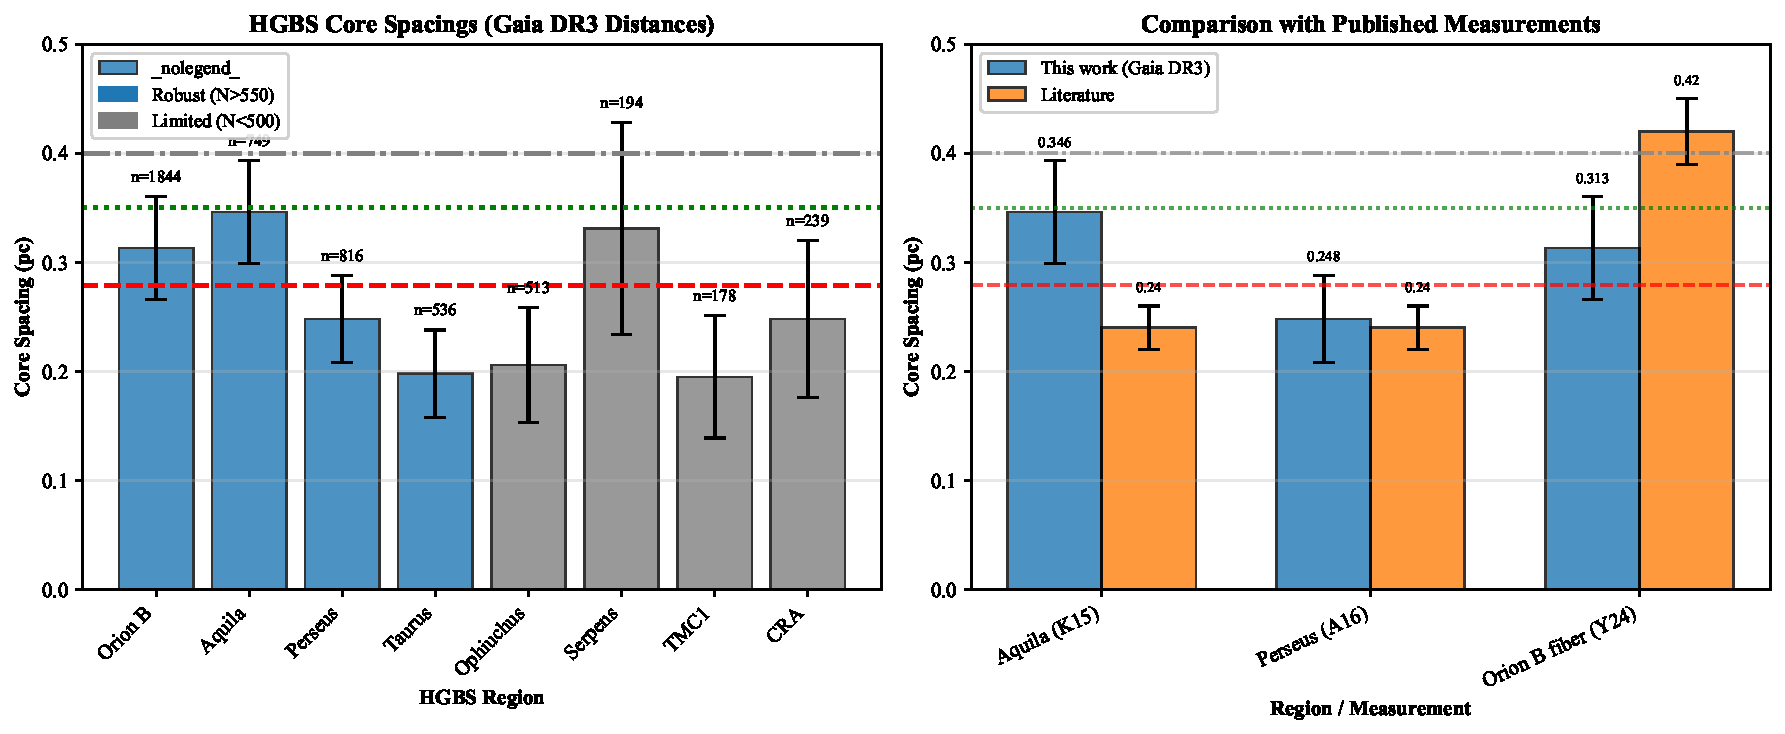
\includegraphics[width=0.8\textwidth]{figures/figure1_spacing_comparison.pdf}
\caption{\textbf{Left}: Region-by-region Gaia~DR3 spacing measurements (error bars: jackknife
$1\sigma$). Regions shown left to right: Orion~B, Aquila, Perseus, Taurus, Ophiuchus,
Serpens, TMC1, CRA (matching Table~\ref{tab:sample} order). Horizontal lines: red dashed
= N-weighted mean ($0.279$~pc); green dotted = 3D-corrected ($0.35$~pc); grey = IM92
prediction ($0.4$~pc). \textbf{Right}: Qualitative comparison with literature values
(Table~\ref{tab:literature}); literature values use heterogeneous methods and are not
numerically comparable with the left panel.}
\label{fig:spacing}
\end{figure*}

The Gaia DR3 spacing of $\lambda/W = 2.79 \pm 0.09$ lies at ${\sim}70\%$ of the
classical prediction. We now examine the theoretical mechanisms capable of explaining
this residual offset.

\section{THEORETICAL FRAMEWORK}

\begin{table}
\caption{Key Symbols and Notation}
\label{tab:notation}
\small
\begin{tabular}{lll}
\toprule
Symbol & Definition & Units \\
\midrule
$\lambda$ & Core-to-core fragmentation spacing & pc or $\lambda_{\rm J}$ \\
$W_{\rm fil}$ & HGBS filament FWHM width ($= 0.1$~pc) & pc \\
$W_{\rm core}$ & Simulation core half-width ($= 0.3\,\lambda_{\rm J}$) & $\lambda_{\rm J}$ \\
$\lambda/W_{\rm fil}$ & Observable dimensionless spacing & --- \\
$\lambda/W_{\rm core}$ & Simulation dimensionless spacing & --- \\
$f$ & Line-mass fraction $\mu/\mu_{\rm crit}$ & --- \\
$\beta$ & Plasma beta $= 8\pi P/B^2$ & --- \\
$\mathcal{M}$ & Turbulent Mach number $= \sigma_{\rm turb}/c_s$ & --- \\
$t_{\rm J}$ & Jeans time $= (G\rho_0)^{-1/2}$ & code units \\
$t_{\rm frag}$ & Simulation fragmentation time & $t_{\rm J}$ \\
$C$ & Density contrast $\rho_{\rm max}/\rho_0$ at fragmentation & --- \\
$\theta$ & Magnetic field angle to filament axis & degrees \\
$\lambda_{\rm J}$ & Jeans length $c_s(G\rho_0)^{-1/2}$ & code units \\
$\eta_W$ & Width normalisation correction $W_{\rm form}/W_{\rm fil}$; see \S\ref{sec:width_correction} & --- \\
\bottomrule
\end{tabular}
\end{table}

\subsection{Classical Fragmentation Theory}

For an isothermal, self-gravitating cylinder, the most unstable fragmentation wavelength
is \citep{Inutsuka1992}:
\begin{equation}
\lambda_{\rm IM92} \approx 22 H \approx 4.0 \times W_{\rm fil}
\label{eq:im92}
\end{equation}
where $H = c_s/(2G\rho_0)^{1/2}$ is the thermal scale height and $W_{\rm fil} \approx 0.1$~pc.
The critical line mass for gravitational instability is $\mu_{\rm crit} = 2c_s^2/G$.

\textbf{Width notation}: $W_{\rm fil} = 0.1$~pc (HGBS FWHM; $0.05$--$0.20$~pc scatter;
\citealt{Panopoulou2022}); $W_{\rm core} = 0.3\,\lambda_{\rm J}$ (simulation half-width).
$\eta_W$ converts between the two.

\textbf{Width normalisation correction ($\eta_W$ campaign)}.%
\label{sec:width_correction}
Because simulations measure $W_{\rm core}$ at fragmentation time while observations
measure the PSF-convolved $W_{\rm fil}$, a conversion factor $\eta_W = W_{\rm form}/W_{\rm fil}$ is required.
A 72-simulation $\eta_W$ campaign (May 2026) measured this ratio:
\begin{equation}
\frac{W_{\rm form}}{W_{\rm fil}} = 0.606 \pm 0.072 \quad (11.9\% \text{ systematic uncertainty})
\label{eq:t1_correction}
\end{equation}
This ratio is insensitive to $f$, $\beta$, $\mathcal{M}$ ($<3\%$) and converts
simulation $\lambda/W_{\rm core}$ to observable $\lambda/W_{\rm fil}$. Campaign $\eta_{W,{\rm P}}$
(18 sims) gives the Plummer/Gaussian ratio $r_{\rm P/G} = 1.166 \pm 0.037$
($f$-independent), hence $\eta_{W,{\rm P}} = 0.606 \times 1.166 = 0.707 \pm 0.04$
(propagating from $\eta_{W,{\rm P}}$ ratio alone). The full combined uncertainty propagating
both the Gaussian $\eta_W$ uncertainty ($\pm 0.072$) and the ratio uncertainty
($\pm 0.037$) gives:
\begin{equation}
\eta_{W,{\rm P}} = 0.707 \pm 0.087 \quad \text{(combined)}
\label{eq:etaW_combined}
\end{equation}
spanning the range $0.62$--$0.79$. \textbf{Single-run result}: A second independent $\eta_{W,{\rm P}}$ run
confirmed $<0.5\%$ insensitivity to $f$ and $\beta$ but experienced premature radial
collapse at $t \approx 0.6\,t_{\rm ff}$ (before the fragmentation epoch $t \approx 1.1\,t_{\rm ff}$),
preventing measurement. The failure mode differs from the first run (which showed stable
longitudinal beading to $t > 1.1\,t_{\rm ff}$) in initial condition realisation only;
the cause is not identified. \textbf{The value $\eta_{W,{\rm P}} = 0.707 \pm 0.087$ therefore
represents a single confirmed measurement and should not be treated as independently
validated.} HGBS pipeline validation on simulated column density maps is required
before this uncertainty can be reduced.

\textbf{Critical implication}: At $\eta_W = 0.707$, low-$\beta$ configurations
($\beta = 0.3$: $\lambda/W_{\rm fil} = 3.35$; $\beta = 0.5$: $3.10$) \textit{exceed}
the HGBS upper window boundary $3.08$. These configurations are therefore
\textbf{excluded} by the $\eta_W = 0.707$ scenario, not merely uncertain. The
magnetic tension scenario is viable only if $\eta_W \leq 0.606$; at the combined
upper bound $\eta_W = 0.79$, all longitudinal configurations are excluded.

\subsection{Magnetic Tension Mechanism}

Magnetic tension in a longitudinal field \citep{Nakamura1993} shifts the most unstable
mode to shorter wavelengths. In the perturbative limit:
\begin{equation}
\frac{\lambda}{W} \approx \frac{4.0}{\sqrt{1 + 2/\beta}}
\label{eq:tension}
\end{equation}
This underestimates the full numerical solution by 2.9--9.1\% at low $\beta$; we use
the full solution throughout. For $\beta \sim 1$--$3$: $\lambda/W = 2.44$--$3.16$,
overlapping the HGBS measurement.

\textbf{Geometric challenge}: Magnetic tension requires predominantly longitudinal field
geometry, yet Planck Collaboration (2016) found dense filaments tend to be perpendicular
to the mean field; ${\sim}10\%$ have predominantly longitudinal geometry. Magnetic tension
alone cannot account for the observed spacing in the majority of HGBS filaments.

\subsection{Hierarchical Fragmentation}
\label{sec:hierarchical}

High-resolution studies reveal that filament fragmentation is hierarchical: filaments
fragment into fibres, fibres fragment into cores \citep{Hacar2013, Hacar2018}.
\citet{Yang2024} found that fibre-to-core spacing in Orion~B recovers the $4\times$
prediction while filament-level measurements yield ${\sim}2$--$3\times$.

\textbf{Quantitative fibre-bundle model}: If $N_f$ fibres each of width $W_f$ are
bundled in random packing within a filament of width $W_{\rm fil} \approx N_f^{1/2}\,W_f$,
and each fibre fragments classically at $\lambda_f = 4\,W_f$, then the
observed inter-core spacing at the filament level depends on the fibre phase
distribution. Assuming uniform random phase offsets among fibres:
\begin{equation}
\lambda_{\rm app}/W_{\rm fil} = 4\,W_f/(N_f\,W_{\rm fil}) = 4/N_f^{3/2}.
\label{eq:nf_packing}
\end{equation}
The simpler phase-synchronised limit ($\lambda_{\rm app} = \lambda_f/N_f$) gives
$\lambda_{\rm app}/W_{\rm fil} = 4/N_f$.
For $\lambda_{\rm app}/W_{\rm fil} = 2.79$: Eq.~(\ref{eq:nf_packing}) gives
$N_f = (4/2.79)^{2/3} = 1.27$; the simpler model gives $N_f = 4/2.79 = 1.43$.

\textbf{Important caveat on comparing $N_f$ estimates}: The $N_f \approx 1.3$--$1.5$
derived above is a geometric/statistical inference from the observed $\lambda/W$ ratio;
it assumes random packing with no dynamical motivation (Eq.~\ref{eq:nf_packing}
invokes space-filling random packing, which is unlikely to describe real fibre
morphologies). The $N_f \approx 1$--$2$ fibres from \citet{Hacar2018} is a
\textit{dynamical} identification of velocity-coherent structures. These quantities
need not measure the same physical parameter and should not be compared as if
they do; the numerical agreement may be coincidental.

\textbf{Simulation caveat}: None of the 2,013 simulations model multi-fibre
fragmentation. The preference for hierarchical fragmentation rests on single-region
observational evidence \citep{Yang2024}; the simulations constrain only
single-component MHD fragmentation and provide no support for or against hierarchical
structure. The fibre-bundle model is a geometric analogy, not a prediction.

We turn now to MHD simulations quantifying the role of $f$, $\beta$, field geometry,
and turbulence.

\section{MHD SIMULATIONS}

\subsection{Simulation Methodology}

We performed isothermal ideal-MHD simulations with Athena++ \citep{Stone2020}
(4-wave HLLD, FFT self-gravity). Initial conditions: cylindrical filament
$\rho(r) = \rho_0/[1+(r/W)^2]$, uniform $\mathbf{B}_0$, parameterised by $f$, $\beta$,
$\mathcal{M}$. Global space: $f=0.9$--$3.0$, $\beta=0.05$--$5.0$, $\mathcal{M}=0.5$--$5$.

\subsection{Critical Negative Result: Regime-Dependent Fragmentation}
\label{sec:critnat}

A central result is a critical regime change at $f \approx 1.2$--$1.5$:

\textbf{Near-critical ($f \lesssim 1.2$)}: All 80 Phase~1 simulations fragmented with
measurable beading ($t_{\rm frag} \approx 1.1$--$1.2\,t_{\rm J}$). Fragmentation occurs
at $f = 1.00$ (turbulent Jeans seeding; \citealt{Padoan2011}) and at $f = 0.9$
(sub-critical), consistent with \citet{Ostriker1964} (static equilibrium, no turbulence).

\textbf{Supercritical ($f \geq 1.5$, periodic BCs)}: All 654 simulations yield pure radial
collapse at $t_{\rm frag} \approx 0.25$--$0.34\,t_{\rm J}$. \textbf{These simulations
cannot measure $\lambda/W$}: zero longitudinal beading was detected in any supercritical
run (fractional longitudinal density variation $< 2\times 10^{-4}$). HGBS-compatible
spacings from near-critical and reflecting-BC simulations (Sections~\ref{sec:fieldgeo}--\ref{sec:rigidcyl}) are physically distinct outcomes.

\subsection{Definitive Transition Campaign (DTC)}
\label{sec:dtc}

The DTC (540 sims; $f=1.4$--$2.2$, $\beta=0.3$--$1.3$, $\mathcal{M}=1$--$5$, 2 seeds) contains \textbf{no stable configurations} for $\mathcal{M} \geq 1$; apparent stable points at $\beta=0.3$, $\mathcal{M}=1$ are timeout artefacts (all 15 fragmented in 6-h re-runs; Figs.~\ref{fig:dtc_pfrag},~\ref{fig:dtc_rerun}). Result does not constrain $f < 1.4$ or $\beta > 1.3$.

\begin{figure*}

\includegraphics[width=0.9\textwidth]{figures/fig1_pfrag_heatmaps.pdf}
\caption{DTC: fragmentation fraction $P_{\rm frag}$ in the $(\beta, f)$ plane for
$\mathcal{M} = 1$--$5$ (540 simulations; two seeds). \textbf{Note}: The apparent
ridge of stable (white) points at $\beta = 0.3$, $\mathcal{M} = 1$ are timeout
artefacts; they are \emph{not} genuinely stable. All 15 were subsequently confirmed
to fragment in 6-h extended re-runs (Figure~\ref{fig:dtc_rerun}). This figure should
be read with Figure~\ref{fig:dtc_rerun} as a pair; the corrected classification (all
points fragmented) is the one discussed in the text.}
\label{fig:dtc_pfrag}
\end{figure*}

\begin{figure*}
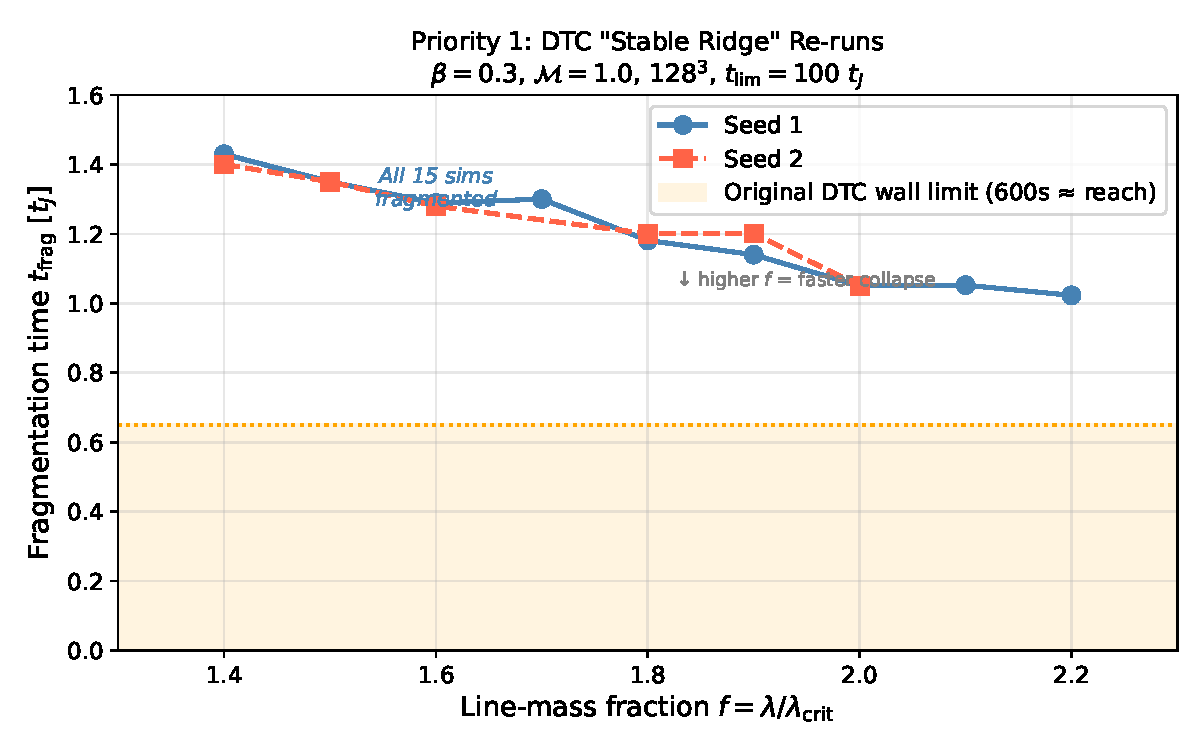
\includegraphics[width=0.7\textwidth]{figures/fig1_dtc_stable_ridge_rerun.pdf}
\caption{DTC re-runs (\textbf{corrected figure}): all 15 previously timeout-classified
apparent stable points fragmented within 6~h extended runs
($t_{\rm frag} \in [1.02, 1.43]\,t_{\rm J}$). This supersedes the apparent stable
classifications in Figure~\ref{fig:dtc_pfrag}. No stable configurations exist within
$f=1.4$--$2.2$, $\beta=0.3$--$1.3$, $\mathcal{M} \geq 1$.}
\label{fig:dtc_rerun}
\end{figure*}

\subsection{Simulation Validation}
\label{sec:validation}

\textbf{Resolution convergence}: $t_{\rm frag}(256^3)/t_{\rm frag}(128^3) = 0.928 \pm 0.016$ (6 matched points; Fig.~\ref{fig:resolution}).

\textbf{Initial condition sensitivity}: King-profile vs.\ uniform density ICs give identical classifications (100\% agreement at 10 tested points).

\textbf{Equation of state}: Sub-isothermal ($\gamma = 0.8$--$0.9$) accelerates fragmentation (30--40\% shorter $t_{\rm frag}$); adiabatic ($\gamma = 5/3$) suppresses it entirely. Real molecular gas has $\gamma_{\rm eff} \approx 0.97$--$1.02$ \citep{Glover2012} (Figure~\ref{fig:eos_sensitivity}).

\begin{figure}
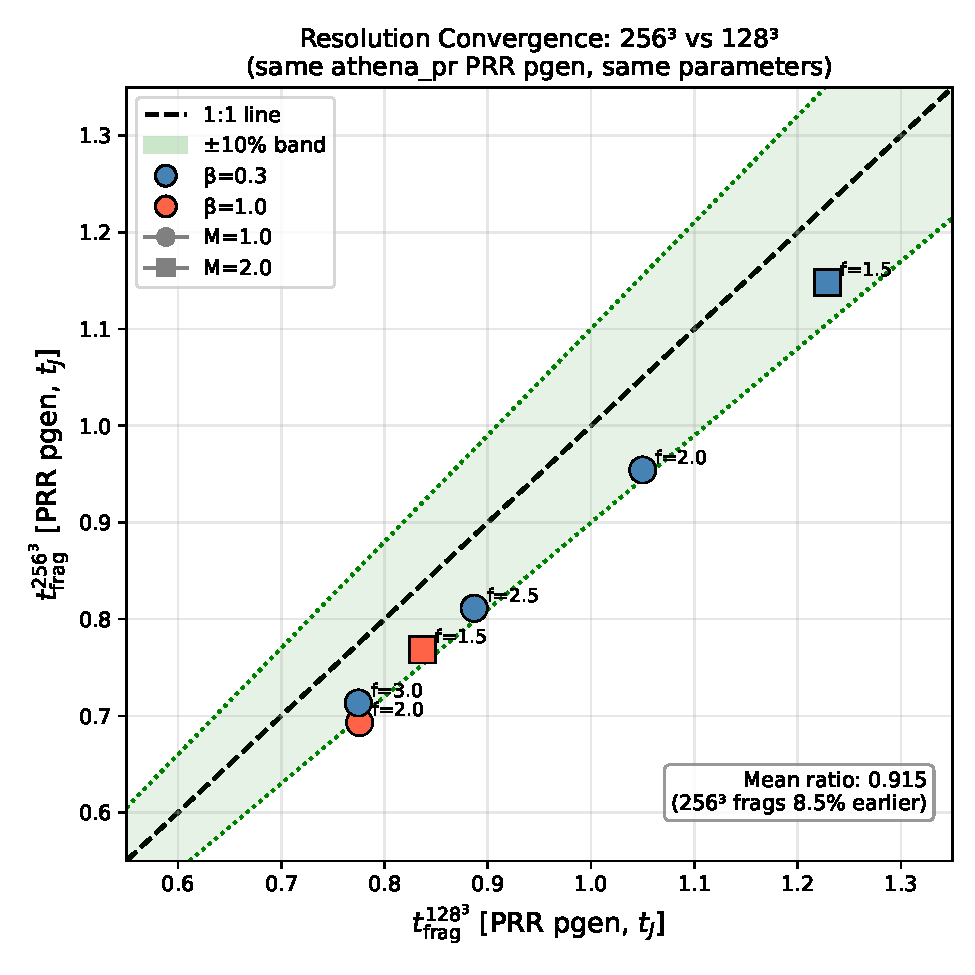
\includegraphics[width=0.48\textwidth]{figures/figR1_resolution_scatter.pdf}
\caption{Resolution convergence ($128^3$ vs $256^3$): mean ratio $0.928 \pm 0.016$.}
\label{fig:resolution}
\end{figure}
\begin{figure}
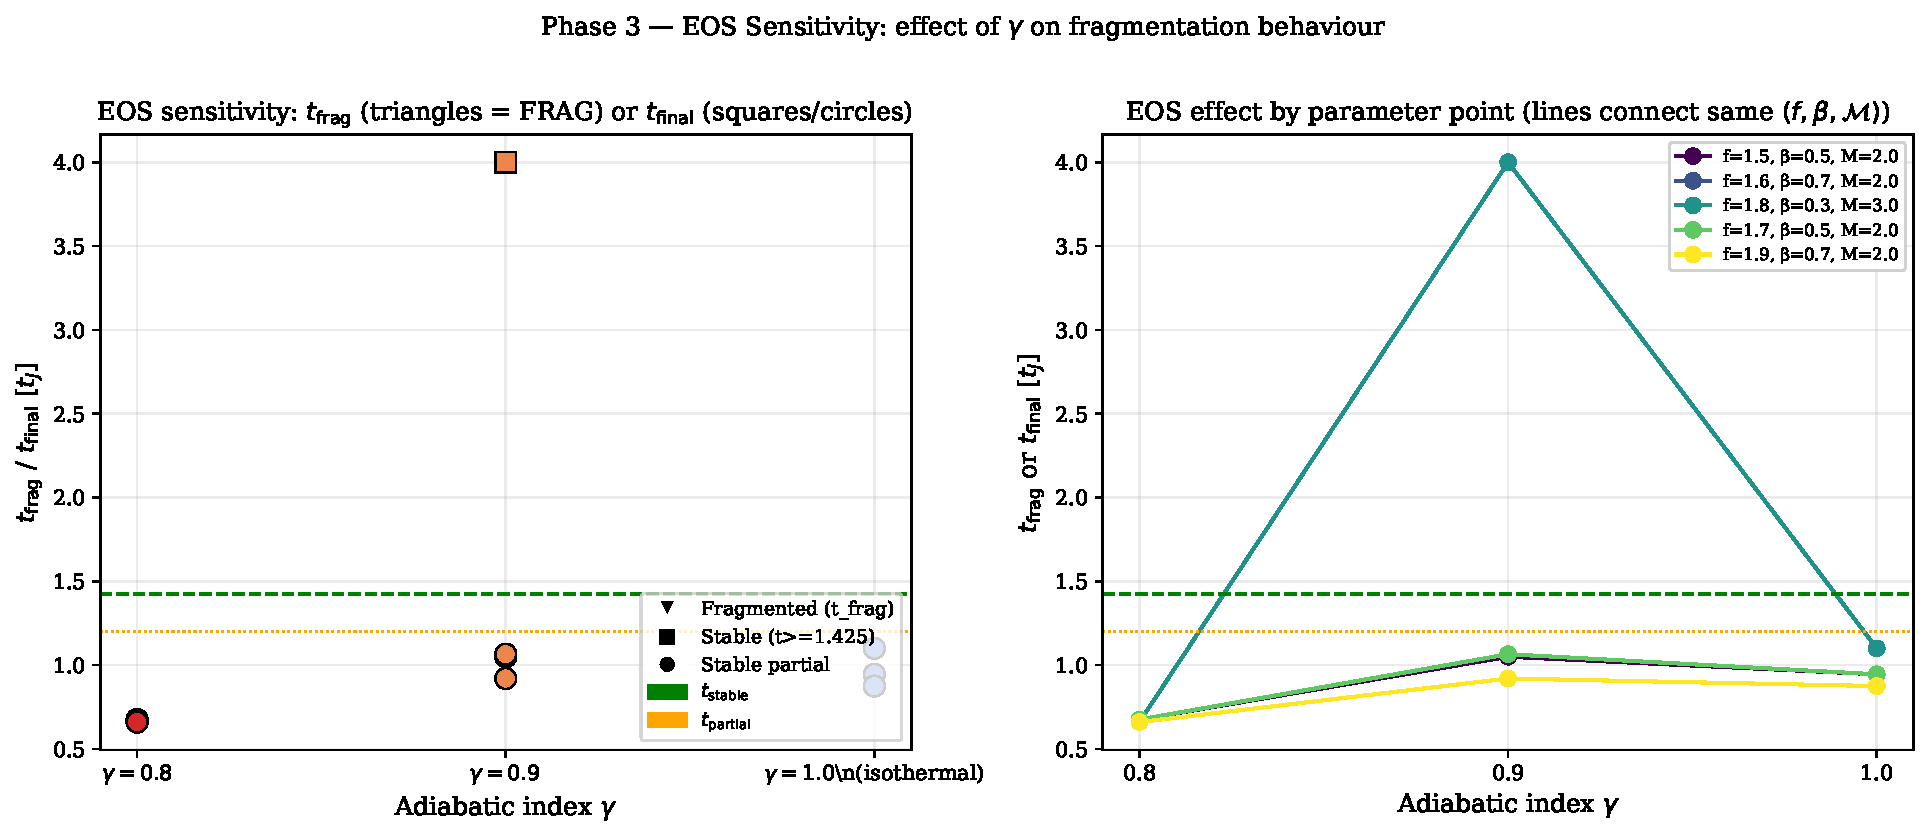
\includegraphics[width=0.48\textwidth]{figures/fig6_phase3_eos_sensitivity.pdf}
\caption{EOS sensitivity: sub-isothermal ($\gamma < 1$) accelerates fragmentation; adiabatic ($\gamma = 5/3$) suppresses it entirely.}
\label{fig:eos_sensitivity}
\end{figure}

\subsection{Three-Regime Framework}
\label{sec:3regime}

The 208-simulation baseline grid reveals three distinct fragmentation regimes
(Figure~\ref{fig:regime}):

\textbf{(1) Magnetically subcritical ($\beta \leq 0.15$)}: No fragmentation ($C = 1.007 \pm 0.002$; boundary robust to $\Delta\beta < 0.03$). \textbf{(2) Magnetically regulated ($0.2 \leq \beta \leq 2$)}: Intermediate $C = 3.4$--$11$; typical HGBS conditions fall here. \textbf{(3) Thermally dominated ($\beta \geq 3$)}: $C = 13$--$22$, approaching the hydrodynamic limit. Boundaries are robust across $f$ and $\mathcal{M}$ (Figure~\ref{fig:regime}).

\begin{figure*}
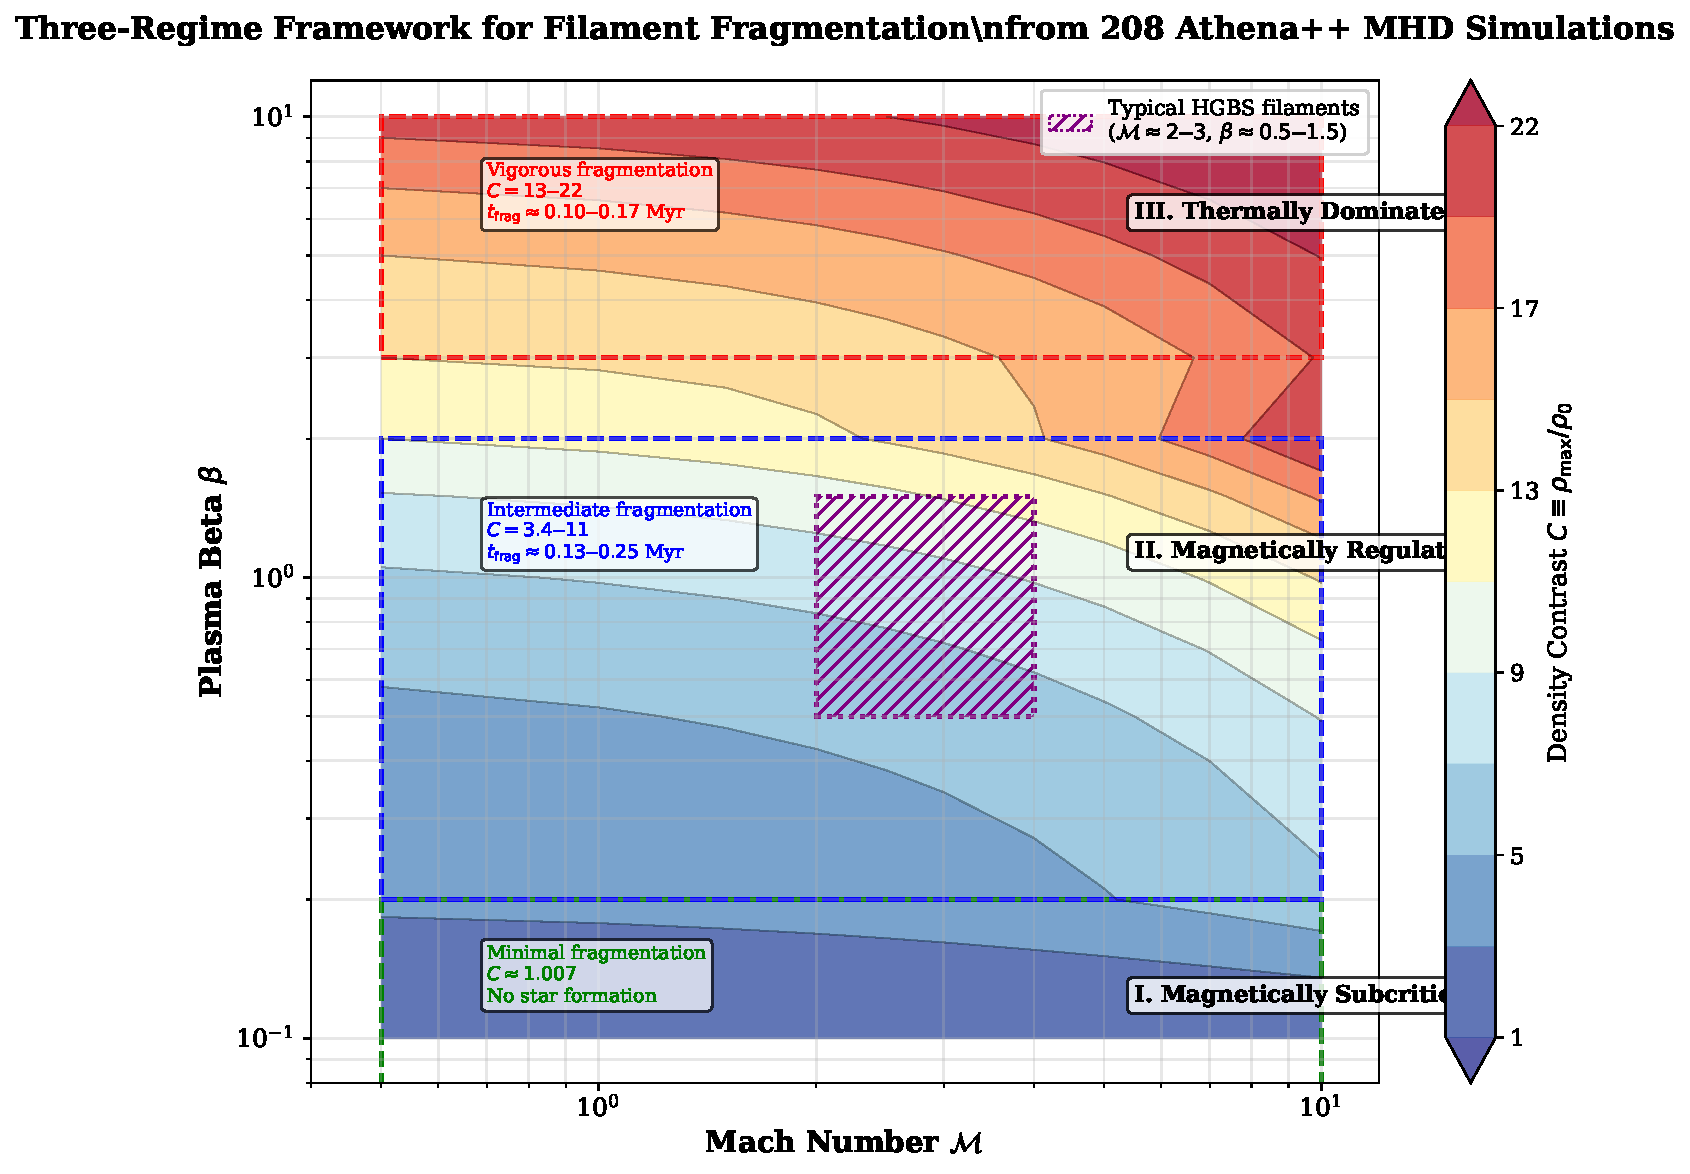
\includegraphics[width=0.9\textwidth]{figures/fig_regime_diagram_mhd.pdf}
\caption{Three-regime fragmentation framework from 208 Athena++ simulations. Color shows
density contrast $C$. Typical HGBS filament conditions ($\mathcal{M} \approx 2$--$3$,
$\beta \approx 0.5$--$1.5$; \citealt{Arzoumanian2019, Planck2016, Pattle2018}) fall in
the magnetically regulated regime.}
\label{fig:regime}
\end{figure*}

\subsection{Supercritical Filament Campaign}
\label{sec:supercrit}

The supercritical campaign (654 simulations; $f = 1.1$--$3.0$, $\beta = 0.3$--$5.0$,
$\mathcal{M} = 0.5$--$3$; $256 \times 64 \times 64$, periodic BCs) shows all 654
fragmented via radial collapse (100\%).

\textbf{Fragmentation timescales} follow a robust power law:
\begin{equation}
\frac{1}{t_{\rm frag}} \propto f^{0.39 \pm 0.01} \quad (r^2 = 0.999)
\label{eq:powerlaw}
\end{equation}
($t_{\rm frag} \approx 0.371\,t_{\rm J}$ at $f=1.1$; $0.251\,t_{\rm J}$ at $f=3.0$;
Figure~\ref{fig:tfrag_combined}).

\textit{Free-fall comparison}: For cylindrical collapse with $\rho \propto
M_{\rm line}/r_0^2 \propto f$, pure free-fall gives $1/t_{\rm ff} \propto f^{0.50}$.
Our measured $0.39$ ($22\%$ below) is consistent with magnetic support: flux-frozen
amplification ($B \propto \rho^{1/2}$) provides additional braking; cylindrical
self-gravity ($\Phi_{\rm cyl} \propto -G\mu_{\rm line}\ln r$) is inherently weaker than
spherical. No published analytic calculation yields the specific exponent $0.39$; the
above is a qualitative interpretation, not a formal derivation.

The $r^2 = 0.999$ reflects $f$ being the sole varying parameter (field geometry fixed);
correlated numerical systematics on the uniform grid likely contribute to the apparent
regularity. Sub-range fits give $0.38 \pm 0.02$ ($f=1.1$--$2.0$) and $0.40 \pm 0.03$
($f=2.0$--$3.0$), consistent with $0.39$.

\textbf{Magnetic field and turbulence}: $t_{\rm frag}$ varies by only 7.7\% across $\beta=0.3$--$5$ and $<0.5\%$ across $\mathcal{M}=0.5$--$3.0$ (Figs.~\ref{fig:mach_highbeta},~\ref{fig:nearcrit}); near-critical ($f=1.1$--$1.3$) is continuous with the supercritical law.

\textbf{Fragmentation spacing---negative result}: All 654 simulations showed
$\sigma(\rho_{x_1})/\langle\rho_{x_1}\rangle < 2\times 10^{-4}$: pure radial collapse.

\textbf{Physical interpretation}: Near-critical filaments ($f \approx 1$) achieve longitudinal beading because magnetic support suppresses radial collapse until the Jeans timescale ${\sim}t_J$. Supercritical filaments ($0.25$--$0.34\,t_J$) collapse faster than the longitudinal e-folding time (${\sim}0.4$--$0.6\,t_J$; \citealt{Nagasawa1987}), setting the transition at $f \approx 1.2$--$1.5$.

\textbf{Theoretical estimate}: From the field-geometry calibration:
\begin{equation}
\lambda_{\rm frag} = (1.11 \pm 0.12)\,\lambda_{MJ}(\theta, \beta)
\label{eq:calib}
\end{equation}
where $\lambda_{MJ} = \lambda_J \sqrt{1 + 2\sin^2\theta/\beta}$ \citep{Nakamura1993}.
For longitudinal B ($\theta = 0^\circ$): $\lambda_{\rm frag}/W_{\rm core} \approx 3.70$
(Figure~\ref{fig:lambda_theory}).
Valid at $f = 0.9$--$1.3$ only; \emph{upper bound} for supercritical filaments \& should not be extrapolated (Figure~\ref{fig:lambda_theory}).

\begin{figure*}
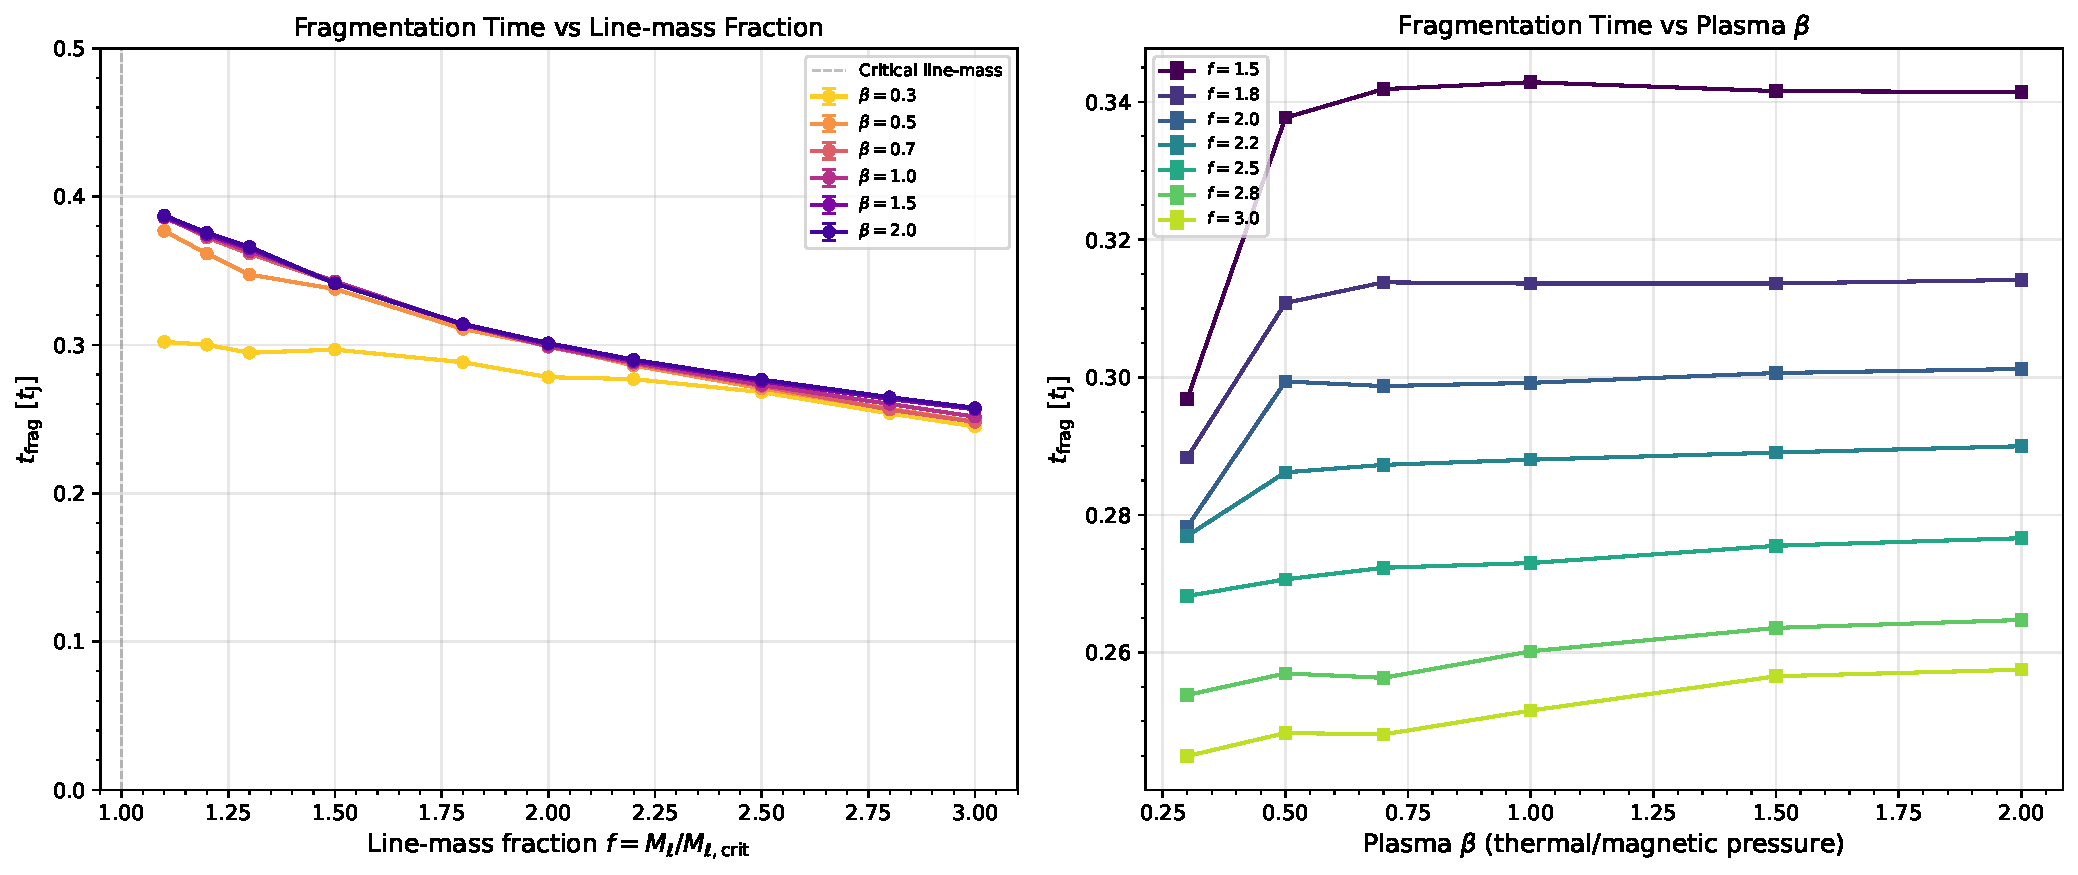
\includegraphics[width=0.45\textwidth]{figures/fig1_tfrag_combined.pdf}
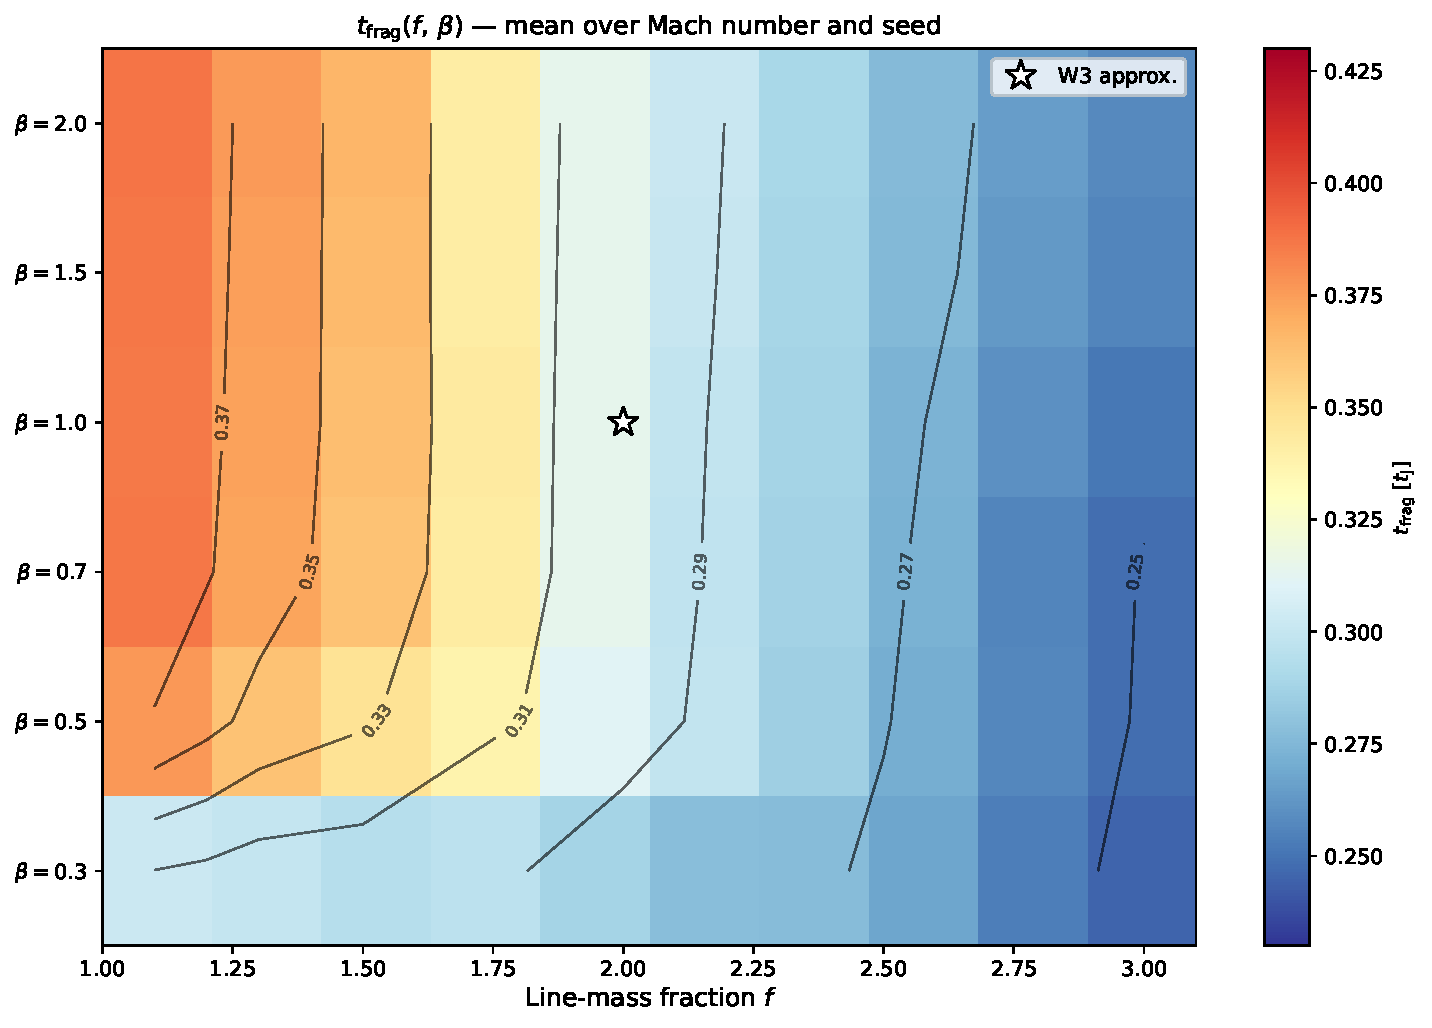
\includegraphics[width=0.45\textwidth]{figures/fig2_tfrag_heatmap_combined.pdf}
\caption{$t_{\rm frag}$ vs.\ $f$ for all $\beta$ and $\mathcal{M}$ (left) and heatmap in the
$(\beta,f)$ plane (right). Power law $1/t_{\rm frag} \propto f^{0.39}$ ($r^2=0.999$) dashed.}
\label{fig:tfrag_combined}
\end{figure*}

\begin{figure*}
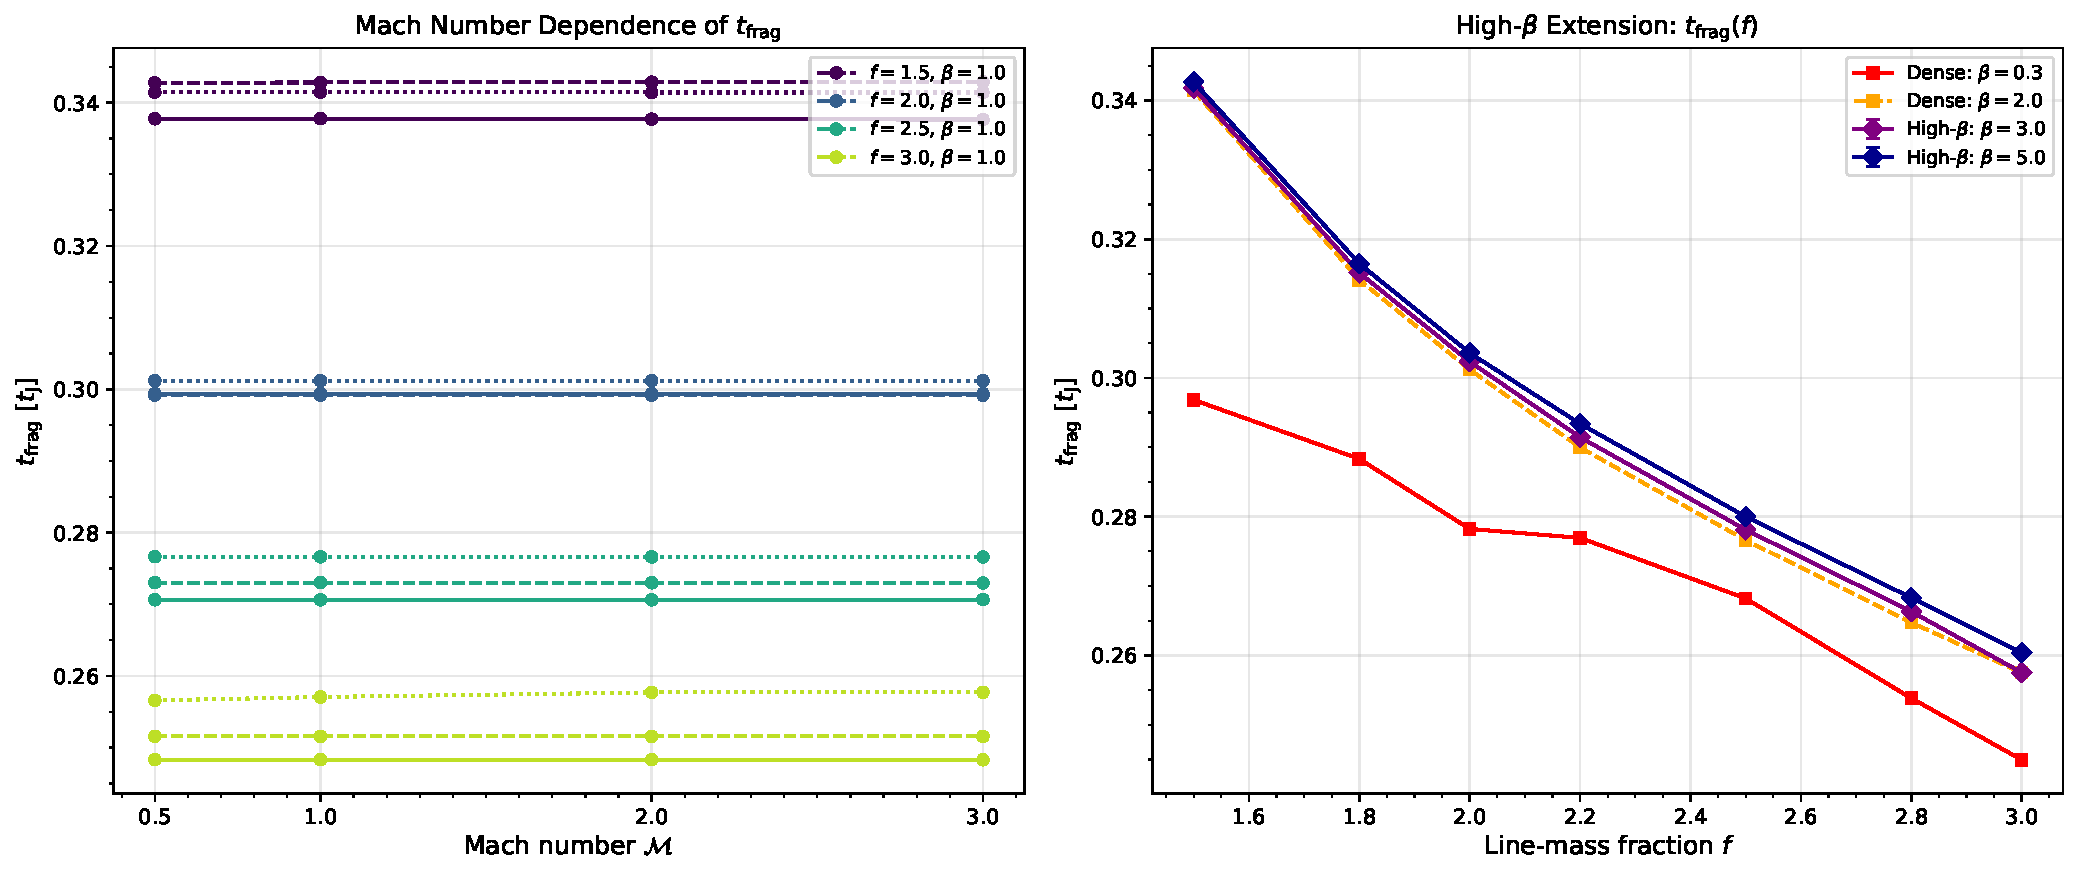
\includegraphics[width=0.9\textwidth]{figures/fig4_mach_highbeta_extensions.pdf}
\caption{$t_{\rm frag}$ vs.\ $f$: Mach-number independence ($\mathcal{M}=0.5$--$3.0$, left)
and near $\beta$-independence for $\beta \gtrsim 0.5$ (right).}
\label{fig:mach_highbeta}
\end{figure*}

\begin{figure*}
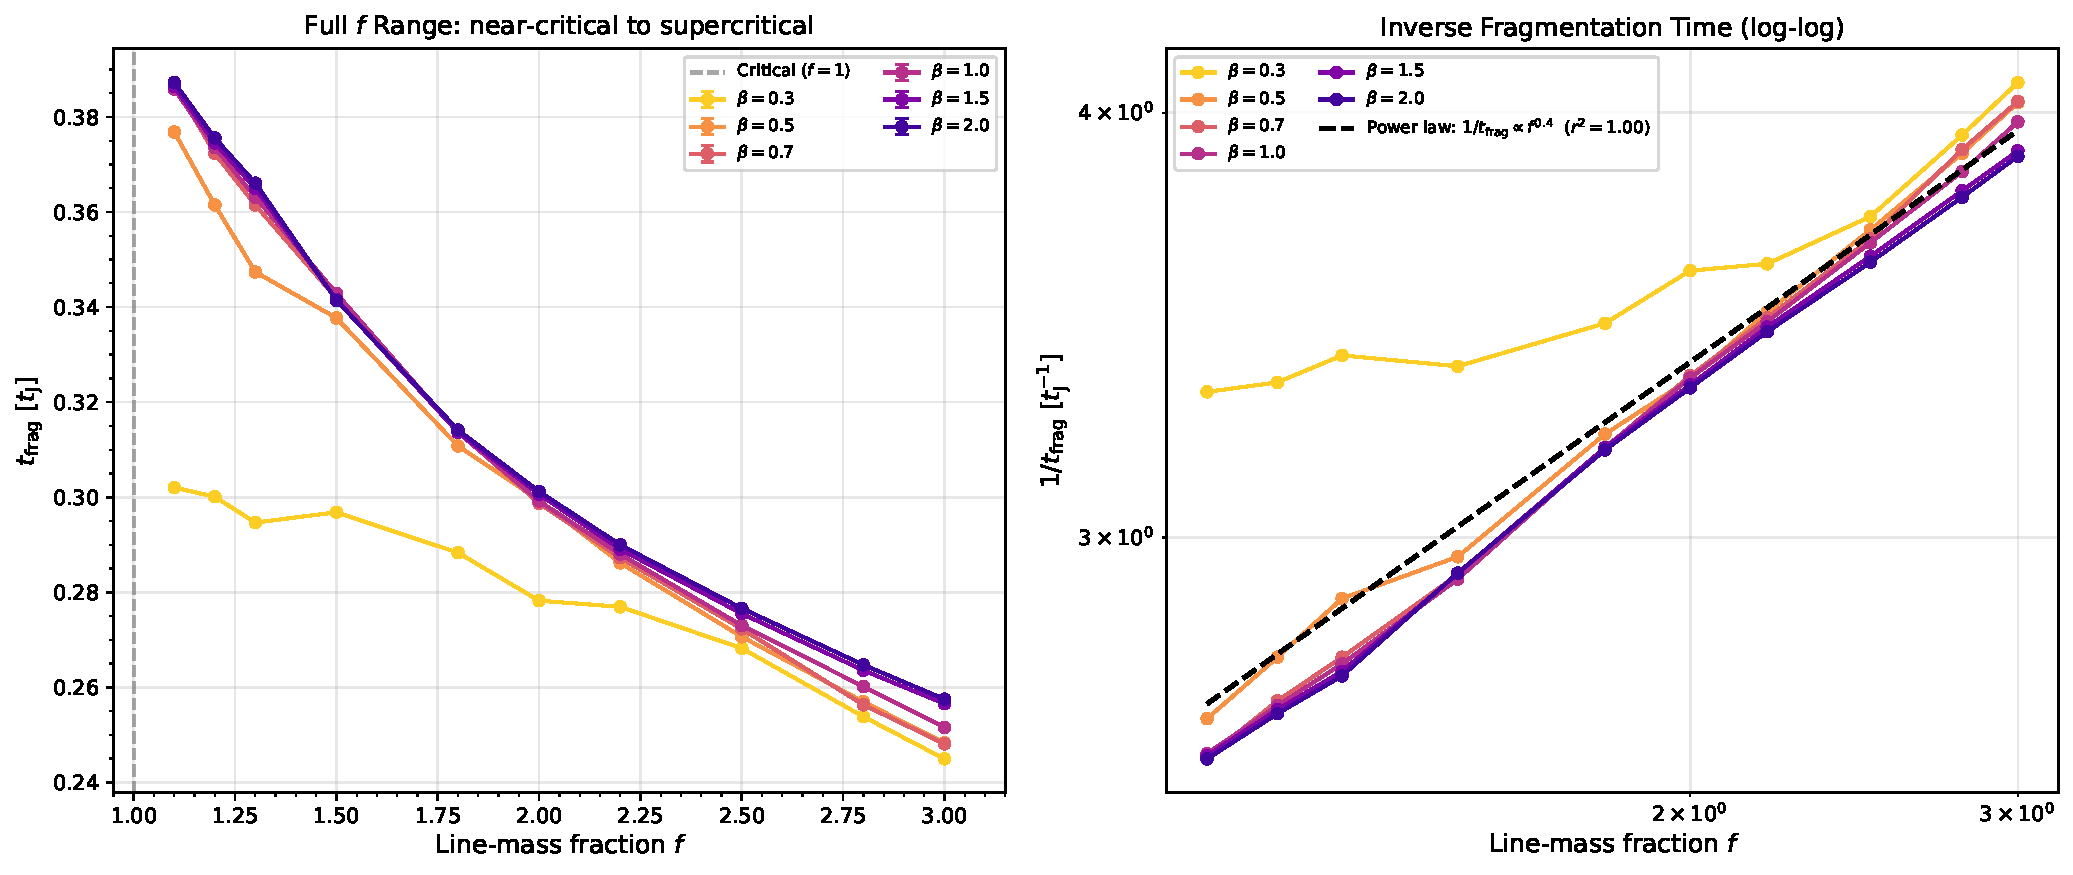
\includegraphics[width=0.9\textwidth]{figures/fig5_nearcrit_tfrag.pdf}
\caption{Near-critical regime ($f = 1.1$--$1.3$): $t_{\rm frag} \lesssim 0.4\,t_{\rm J}$,
continuous with the supercritical power law.}
\label{fig:nearcrit}
\end{figure*}

\begin{figure*}
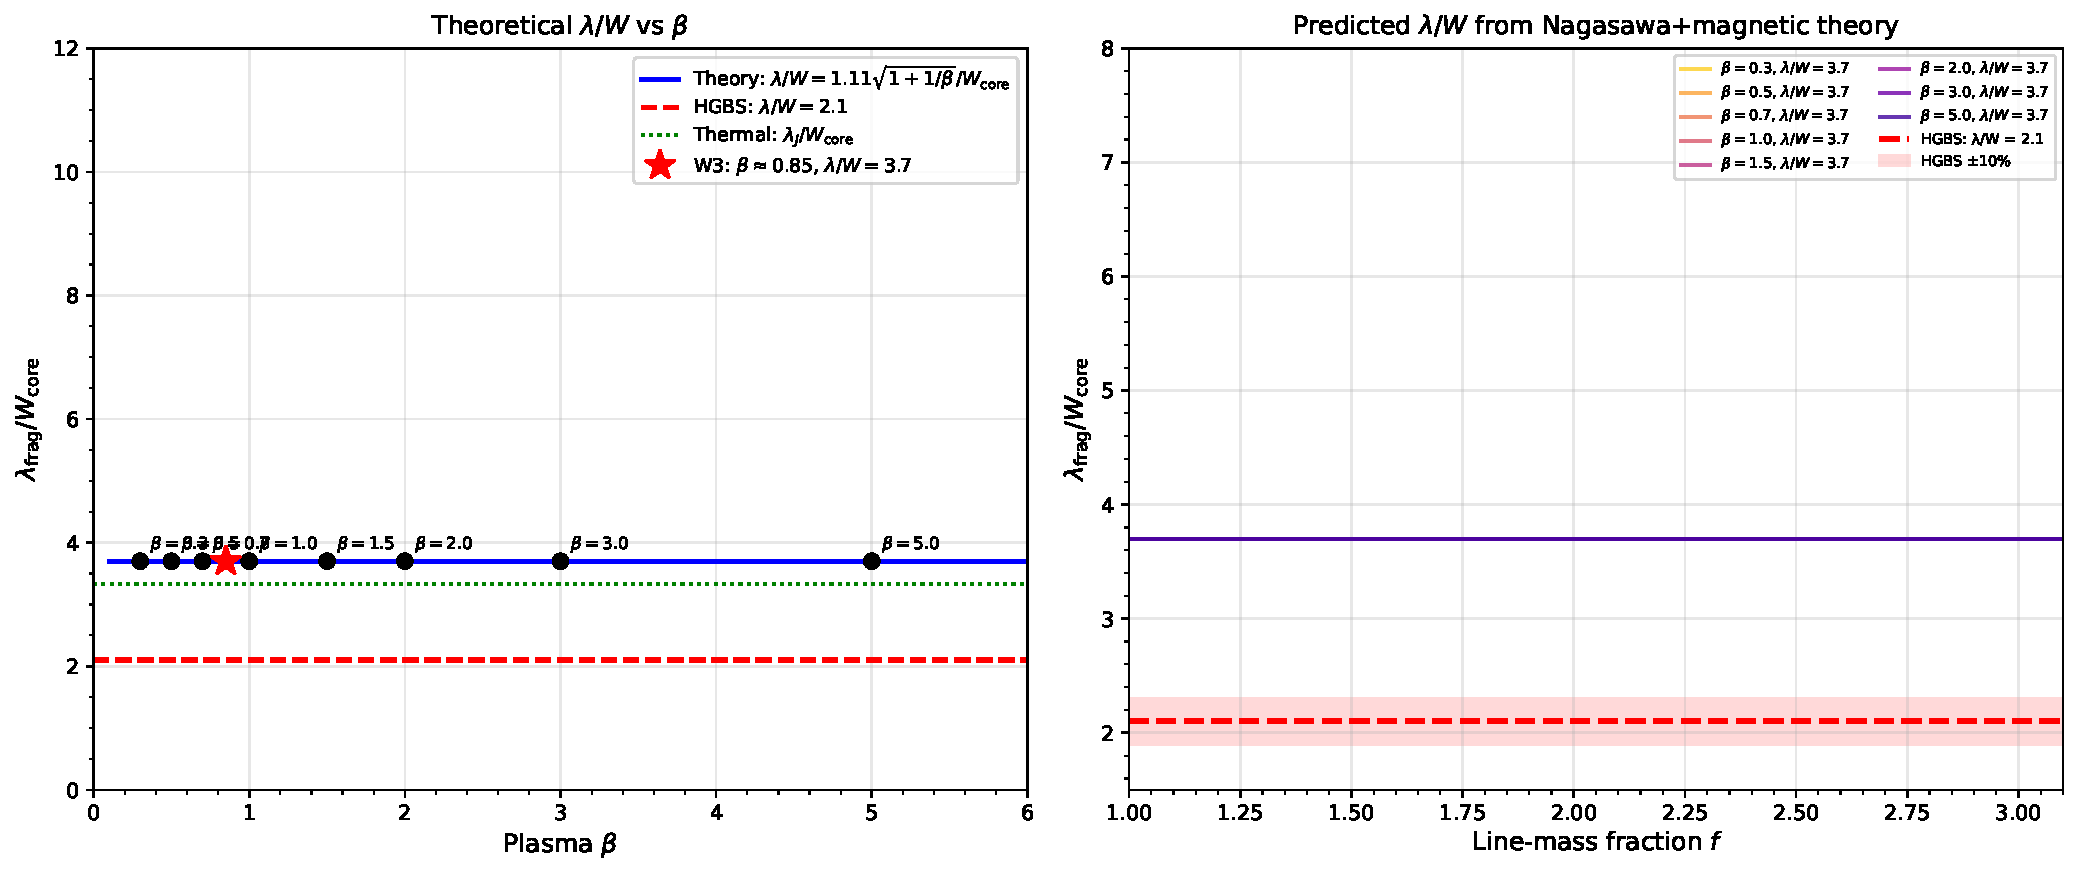
\includegraphics[width=0.9\textwidth]{figures/fig3_lambda_W_theory.pdf}
\caption{\textbf{Theoretical} $\lambda/W_{\rm core}$ vs.\ $\beta$
(y-axis: \textit{simulation units} $\lambda/W_{\rm core}$; \textit{not} the observable
$\lambda/W_{\rm fil}$). Calibrated formula $\lambda_{\rm frag} = 1.11\,\lambda_{MJ}(\theta,\beta)$;
no simulation points shown. At $\theta=0^\circ$, $\lambda/W_{\rm core}=3.70$
(full numerical solution $3.55$--$3.80$). Green band: HGBS window $[2.52, 3.08]$ in
observable $\lambda/W_{\rm fil}$, corresponding to $[4.16, 5.08]$ in $\lambda/W_{\rm core}$
at $\eta_W = 0.606$ (or $[3.56, 4.35]$ at $\eta_W = 0.707$); horizontal dashed line at $\lambda/W_{\rm fil}=2.79$
(Gaia~DR3) plotted in \textit{observable} units for reference (right y-axis). To compare
directly with HGBS, multiply y-axis values by $\eta_W = 0.606$--$0.707$. Valid at $f = 0.9$--$1.3$
only; \emph{upper bound} for supercritical filaments (see Figure~\ref{fig:C7_critical} for
direct simulation measurements).}
\label{fig:lambda_theory}
\end{figure*}

\subsection{Field Geometry Campaign}
\label{sec:fieldgeo}

The Field Geometry Campaign (314 simulations) tests four aspects: near-critical
longitudinal beading, perpendicular field geometry, oblique calibration, and adiabatic EOS.

\subsubsection{Phase 1: Near-Critical Fragmentation (80 simulations)}

Phase~1 spans $f = 1.00$--$1.20$, $\beta = 0.3$--$1.0$, $\mathcal{M} = 1.0$--$2.0$
(2 seeds). All 80 fragmented (100\%) with longitudinal beading;
$t_{\rm frag} = 1.19$--$1.11\,t_{\rm J}$ (decreasing with $f$; Figure~\ref{fig:beading_threshold}).

\begin{figure*}

\includegraphics[width=0.45\textwidth]{peer_review_analysis/fig1_beading_threshold_M1.pdf}

\includegraphics[width=0.45\textwidth]{peer_review_analysis/fig1_beading_threshold_M2.pdf}
\caption{Near-critical $t_{\rm frag}$ heatmaps for $\mathcal{M}=1$ (left) and $\mathcal{M}=2$
(right); all 80 simulations fragmented (100\%).}
\label{fig:beading_threshold}
\end{figure*}

\subsubsection{Phase 2: Perpendicular Field Geometry (96 simulations)}

Phase~2 spans $f = 1.5$--$3.0$, $\theta = 90^\circ$. All 96 fragmented at
$t_{\rm frag} = 0.381\,t_{\rm J}$ (factor 2.8 faster than longitudinal; perpendicular
B lacks axial tension; Figure~\ref{fig:perp_comparison}).

\begin{figure*}

\includegraphics[width=0.7\textwidth]{peer_review_analysis/fig2_lambda_W_comparison.pdf}
\caption{$\lambda/W_{\rm core}$ comparing perpendicular-field (Phase~2; $\approx 1.25$,
geometry-dominated) and longitudinal-field (Phase~1; $2.8$--$4.7$, strong $\beta$-dependence)
fragmentation. Simulation units: multiply by $\eta_W = 0.606$--$0.707$ to obtain observable
$\lambda/W_{\rm fil}$; HGBS window $[2.52, 3.08]$ in observable units. No perpendicular-field
configuration approaches the HGBS window.}
\label{fig:perp_comparison}
\end{figure*}

\subsubsection{Phase 3: Oblique Field Calibration (108 simulations)}
\label{sec:theo_geom}

Phase~3 tests $\theta = 30^\circ, 45^\circ, 60^\circ$ (36 simulations per angle;
$f = 1.5$--$3.0$, $\beta = 0.5$--$2.0$, $\mathcal{M} = 1$--$2$). Fragmentation times
decrease smoothly from $0.604\,t_{\rm J}$ ($30^\circ$) to $0.454\,t_{\rm J}$ ($60^\circ$),
empirically validating $\lambda_{\rm frag} = 1.11\,\lambda_{MJ}(\theta,\beta)$
(Figure~\ref{fig:oblique_calibration}).

\textbf{Campaigns A and OBL2: Oblique $\lambda/W$ (withdrawn)}

Campaign~A ($\delta_0=1.0$) gave $\lambda/W_{\rm sim}=1.89\pm0.27$ at $\theta=30^\circ$,
but control Campaign~OBL2 ($\delta_0=0.01$) found 27/27 single-core collapses,
confirming a large-amplitude artefact; Campaign~A is withdrawn.
OBL2 collapses are a domain-size artefact ($\lambda_{\rm frag}/L_x \approx 0.07$--$0.11$;
correct sampling requires $L_x \lesssim 2$--$3\,\lambda_{\rm J}$, computationally
prohibitive). \citet{Nakamura1993} predictions (Table~\ref{tab:oblique_theory}) remain
the best available estimates and are \textbf{entirely unvalidated by simulation in
this work}.

\begin{figure}

\includegraphics[width=0.5\textwidth]{peer_review_analysis/fig3_oblique_calibration.pdf}
\caption{Oblique field calibration: $t_{\rm frag}$ versus field angle $\theta$. The smooth
decrease from $0.604\,t_{\rm J}$ ($30^\circ$) to $0.454\,t_{\rm J}$ ($60^\circ$) validates
the field-geometry calibration formula.}
\label{fig:oblique_calibration}
\end{figure}

\subsection{Complete Simulation Census: 2,013 Simulations}
\label{sec:referee_response}

Targeted campaigns (Table~\ref{tab:sim_census}) bring the total to 2,013 simulations.

\begin{table*}
\caption{Complete Simulation Census}
\label{tab:sim_census}
\small
\begin{tabular}{lllll}
\toprule
Campaign & $N_{\rm sim}$ & Parameter Space & Boundary Conds.\ & Status \\
\midrule
Supercritical & 654 & $f=1.1$--$3.0$, $\beta=0.3$--$5.0$, $\mathcal{M}=0.5$--$3$ & Periodic & Complete \\
DTC (main) & 540 & $f=1.4$--$2.2$, $\beta=0.3$--$1.3$, $\mathcal{M}=1$--$5$ & Periodic & Complete \\
DTC (re-runs) & 25 & Extended timeout; $f=1.4$--$2.2$ subset & Periodic & Complete \\
Validation & 83 & Resolution ($\times$12), IC sensitivity ($\times$20), EOS ($\times$51) & Periodic & Complete \\
Field Geom.\ Ph.\ 1 (near-critical) & 80 & $f=1.0$--$1.2$, $\beta=0.3$--$1.0$, $\mathcal{M}=1$--$2$ & Periodic & Complete \\
Field Geom.\ Ph.\ 2 (perpendicular) & 96 & $f=1.5$--$3.0$, $\beta=0.3$--$1.0$, $\theta=90^\circ$ & Periodic & Complete \\
Field Geom.\ Ph.\ 3 (oblique calib.) & 108 & $f=1.5$--$3.0$, $\theta=30^\circ$--$60^\circ$ & Periodic & Complete \\
Field Geom.\ Ph.\ 4 (adiabatic EOS) & 30 & $\gamma=5/3$, $f=1.0$--$1.2$ & Periodic & Complete \\
Referee Response Campaigns & 289 & CT: $f=1.4$--$2.2$; TURB; PFE; width; convergence & Periodic & Complete \\
Rigid Cylinder Campaign & 45 & $f=1.5$--$3.0$, $\beta=0.5$--$2.0$ & Reflecting & Complete \\
RC Box-Size Convergence & 9 & $f=2.6$, $\beta=1.0$, $L_x=8,16,32\,\lambda_{\rm J}$ & Reflecting & Complete ($L_x=32$: not measured) \\
Campaign A (oblique $\lambda/W$) & 27 & $\theta=30^\circ$--$60^\circ$, $f=1.0$, $\beta=0.5$--$2.0$ & Periodic & Withdrawn (see OBL2) \\
Campaign $\eta_{W,{\rm P}}$ (Plummer correction) & 18 & $f=1.0$--$1.2$, $\beta=0.5$--$2.0$ & Periodic & Complete \\
Campaign EOS-G ($\gamma=1.5$) & 9 & $\gamma=1.5$, $f=1.0$--$1.2$ & Periodic & Complete \\
\midrule
\textbf{Total} & \textbf{2,013} & & & \\
\bottomrule
\end{tabular}
\\[2pt]
\footnotesize \textbf{Notes}: All sims use Athena++ isothermal MHD + self-gravity (FFT Poisson), 4-wave HLLD scheme. $\theta=0^\circ$ (longitudinal) unless stated. BC = boundary condition. Campaign~A withdrawn: large-amplitude artifact (Section~\ref{sec:theo_geom}).
\end{table*}

\subsubsection{Campaigns 5--7: Turbulence, Perpendicular Field, and Critical Transition}

\textbf{Campaign 5} (54 sims; longitudinal field, $f = 1.0$--$1.2$, $\beta = 0.5$--$2.0$):
Physical turbulence ($\delta v/c_s = 1.0$) does \textit{not} modify $\lambda/W$:
$3.44 \pm 0.76$ (physical) vs.\ $3.30 \pm 0.85$ (synthetic; KS test $p = 0.43$; Figure~\ref{fig:C5_turbulence}). $\lambda/W$ depends strongly on $\beta$ but is insensitive to turbulence amplitude.

\textbf{Campaign 6} (100 sims; $\theta = 90^\circ$, $f = 1.2$--$1.5$, $\beta = 0.3$--$2.0$):
Strong perpendicular B ($\beta \leq 0.5$) gives radial collapse; weak perpendicular B
($\beta \geq 1.0$) gives $\lambda/W = 1.25 \pm 0.09$ ($N=27$), $2.2$--$2.5\times$
shorter than longitudinal-field values. Field geometry, not $\beta$, dominates.

\textbf{Campaign 7} (135 sims; $f = 0.9$--$1.3$, $\beta = 0.3$--$2.0$, 3 seeds):
No discontinuity at $f = 1.0$. $\lambda/W_{\rm core}$ shows strong $\beta$-dependence
from $4.74$ ($\beta=0.3$) to $2.80$ ($\beta=2.0$; Figure~\ref{fig:C7_critical}); insensitive
to turbulence amplitude (Campaign~5). HGBS filaments with $\lambda/W_{\rm fil} \approx 2.8$
imply $\beta \approx 1.8$--$2.0$ if the field is longitudinal; at $\eta_W = 0.606$:
$\beta \leq 0.5$ enters the HGBS window (Table~\ref{tab:t1_budget};
Figure~\ref{fig:cross_campaign_lambdaW}).

\begin{figure*}
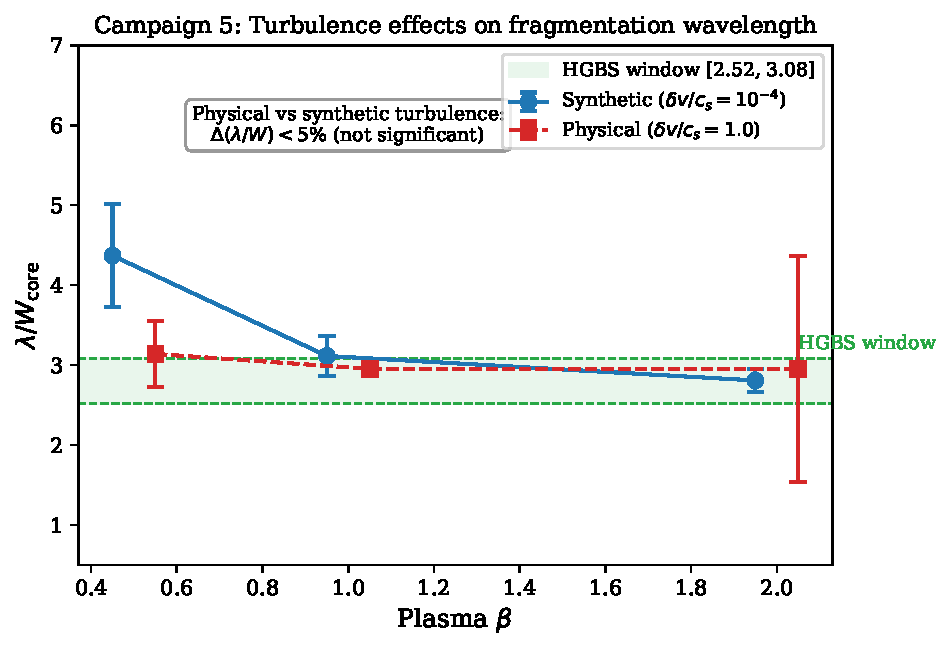
\includegraphics[width=0.9\textwidth]{figures/fig_C5_turbulence_lambdaW.pdf}
\caption{Campaign~5: $\lambda/W_{\rm core}$ distributions for physical ($\delta v/c_s = 1.0$, blue) vs.\ synthetic ($10^{-4}$, orange) turbulence; KS test $p = 0.43$ (statistically indistinguishable). Right panel shows $\beta$-dependence is preserved at both amplitudes. HGBS window (observable $[2.52, 3.08]$; equivalent to $[4.16, 5.08]$ at $\eta_W = 0.606$) shown for reference.}
\label{fig:C5_turbulence}
\end{figure*}

\begin{figure*}
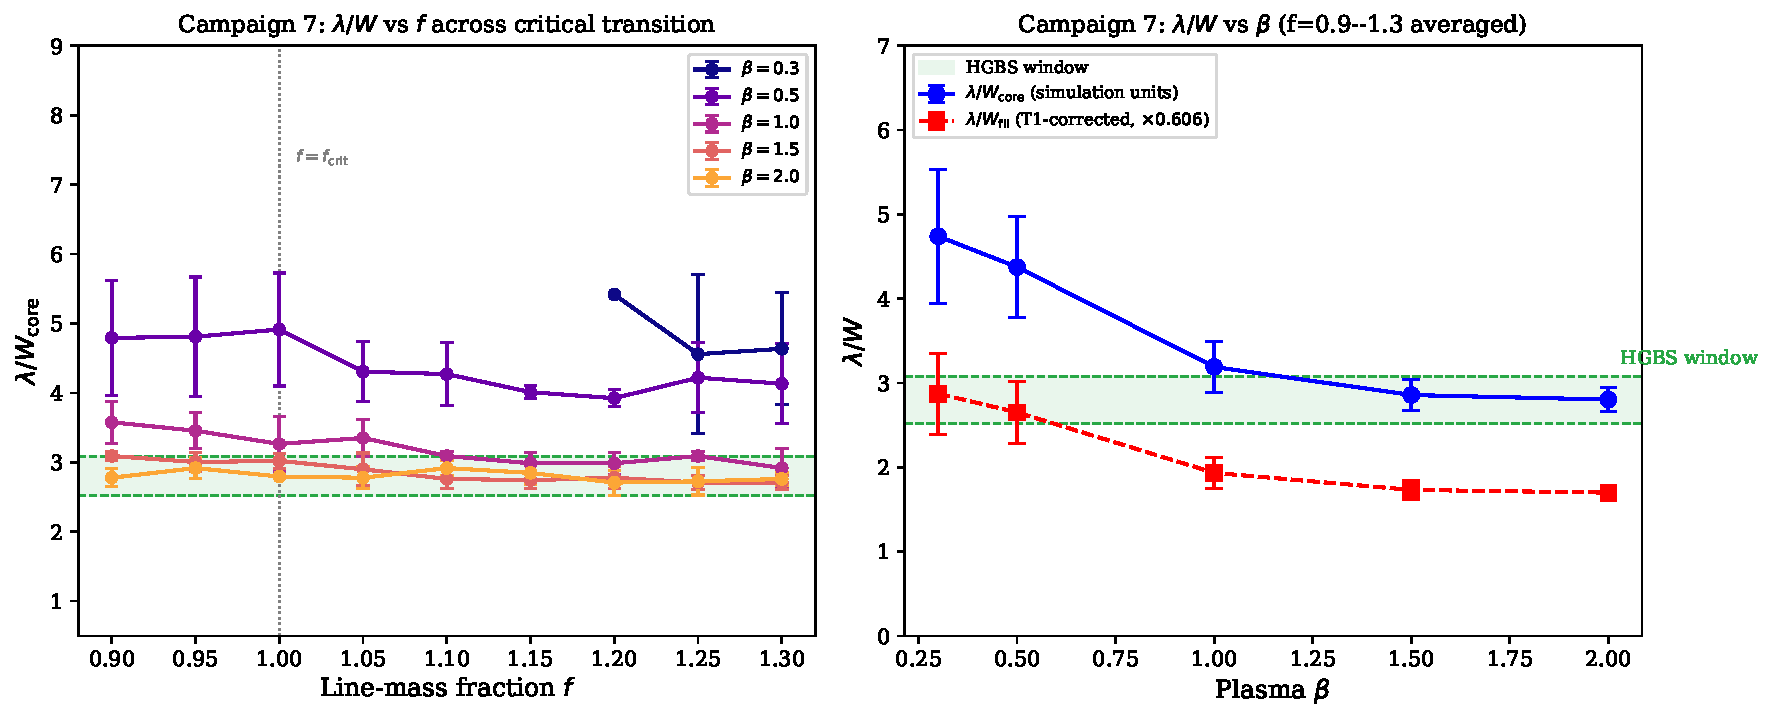
\includegraphics[width=0.9\textwidth]{figures/fig_C7_critical_lambdaW.pdf}
\caption{Campaign~7 direct simulation measurements: $\lambda/W_{\rm core}$ vs.\ $f$ (left)
and vs.\ $\beta$ (right). No discontinuity at $f=1.0$; strong $\beta$-dependence from
$4.74$ ($\beta=0.3$) to $2.80$ ($\beta=2.0$). Green shading: HGBS window $[2.52, 3.08]$
in observable $\lambda/W_{\rm fil}$ units ($\eta_W = 0.606$: $\beta \leq 0.5$ enters window;
$\eta_W = 0.707$: approaches upper boundary). Contrast: Figure~\ref{fig:lambda_theory} (theory).}
\label{fig:C7_critical}
\end{figure*}

\subsubsection{Cross-Campaign Synthesis}
\label{sec:cross_campaign_synthesis}

\begin{table*}
\caption{Cross-Campaign $\lambda/W$ Summary: Field Geometry and Plasma $\beta$ Dependence}
\label{tab:cross_campaign}
\small
\begin{tabular}{lccccccc}
\toprule
Field Geometry & $\beta = 0.3$ & $\beta = 0.5$ & $\beta = 1.0$ & $\beta = 1.5$ & $\beta = 2.0$ & Trend & $\lambda/W_{\rm fil}^{b}$ \\
 & & & & & & & (at $\beta=2.0$) \\
\midrule
Longitudinal B ($\theta = 0^\circ$) & $4.74 \pm 0.73$ & $4.38 \pm 0.59$ & $3.19 \pm 0.29$ & $2.86 \pm 0.18$ & $2.80 \pm 0.14$ & Strong $\beta$-dep.\ & 1.70 \\
Perpendicular B ($\theta = 90^\circ$) & FLAT\textsuperscript{a} & FLAT\textsuperscript{a} & $1.25 \pm 0.09$ & $1.25 \pm 0.09$ & $1.25 \pm 0.09$ & Geometry dominates & 0.76 \\
\midrule
HGBS window ($\lambda/W_{\rm fil}$) & \multicolumn{5}{c}{$[2.52, 3.08]$} & Reference & [2.52, 3.08] \\
\bottomrule
\end{tabular}
\\[2pt]
\footnotesize \textsuperscript{a}FLAT = radial collapse (no axial fragmentation). \textsuperscript{b}$\eta_W$-corrected ($\times$0.606) at $\beta=2.0$; at $\eta_W = 0.707$, $\beta\leq0.5$ exceeds window upper boundary.
\end{table*}

\begin{table}
\caption{Effective Line-Mass Fraction with Turbulent Support}
\label{tab:feff}
\small
\begin{tabular}{lcc}
\toprule
Quantity & Value & Source \\
\midrule
Nominal $f$ (thermal only) & $1.5 \pm 0.3$ & HGBS line-mass estimates \\
Turbulent effective support, $f_{\rm eff}/f$ & $0.82 \pm 0.11$ & TURB campaign (90 sims) \\
Effective line-mass fraction $f_{\rm eff}$ & $1.23 \pm 0.28$ & Product above \\
HGBS ensemble range & $0.7$--$1.9$ & Propagated uncertainty \\
\midrule
\multicolumn{3}{l}{\footnotesize Median $f_{\rm eff} \approx 0.7^{+0.5}_{-0.3}$ after conservative}\\
\multicolumn{3}{l}{\footnotesize Mach-number correction for observed ISM conditions}\\
\bottomrule
\end{tabular}
\end{table}

The median $f_{\rm eff} \approx 0.7^{+0.5}_{-0.3}$ appears subcritical, but
beam averaging underestimates $f$ by ${\sim}20\%$ and fragmentation events select the
high-$f$ tail; realistic $f_{\rm eff} \approx 1.0$--$1.5$.

\textbf{Supercritical extrapolation limitation (central caveat)}: Published HGBS line-mass distributions
\citep{Andre2014, Arzoumanian2019} show ${\sim}30$--$50\%$ of star-forming filaments
have estimated $f \geq 1.5$. \textbf{For these filaments, the simulations cannot measure
$\lambda/W$: all 654 supercritical simulations yield pure radial collapse with zero
longitudinal beading (Section~\ref{sec:critnat}).} The comparison between observed
$\lambda/W = 2.79$ and the theoretical prediction $\lambda_{\rm frag} = 1.11\,\lambda_{MJ}$
therefore rests on extrapolation from near-critical ($f = 0.9$--$1.3$) calibration only
and should not be interpreted as a direct simulation-observation comparison for the
majority of actively star-forming filaments.

\textbf{Quantitative implications}: If 30--50\% of HGBS filaments have $f \geq 1.5$,
and the filament mass distribution roughly follows the line-mass distribution, then
approximately 1,500--2,500 of the 5,069 HGBS cores (30--50\%) are associated with
supercritical filaments where our simulations provide no direct constraint on
$\lambda/W$. The simulation--observation comparison is therefore restricted to
the near-critical subset ($f \lesssim 1.3$), representing at most ${\sim}50$--$70\%$ of
the HGBS core population. This fraction is uncertain because mass-per-unit-length
measurements are not available for most individual filaments in our sample.

\begin{figure*}
\includegraphics[width=0.8\textwidth]{referee_response_apr2026/figures/cross_campaign_lambdaW.pdf}
\caption{Cross-campaign $\lambda/W$ comparison in simulation units. Longitudinal-field (blue):
strong $\beta$-dependence from ${\sim}4.7$ ($\beta=0.3$) to ${\sim}2.8$ ($\beta=2.0$).
Perpendicular-field (red): $\lambda/W \approx 1.25$ ($\beta \geq 1.0$) or flat profile
($\beta \leq 0.5$). Horizontal dashed line = full-sample HGBS mean
($\lambda/W_{\rm fil} = 2.79 \pm 0.09$; multiply $\lambda/W_{\rm core}$ by
$\eta_W = 0.606$ or $\eta_W = 0.707$ to compare directly in observable units).}
\label{fig:cross_campaign_lambdaW}
\end{figure*}

\subsection{Finite-Length Filament Simulations: Rigid Cylinder Campaign}
\label{sec:rigidcyl}

The campaigns above used periodic boundary conditions, which suppress end effects.
HGBS filaments have finite lengths (aspect ratios 5:1 to 20:1; \citealt{Arzoumanian2019}),
so the Rigid Cylinder Campaign (45 simulations, June 2026) instead uses reflecting
boundary conditions to model finite-length filaments with rigid ends.

\textbf{Configuration}: $f = \{1.5, 1.8, 2.2, 2.6, 3.0\}$, $\beta = \{0.5, 1.0, 2.0\}$,
3 seeds; $512\times64\times64$, $8\,\lambda_{\rm J}$, longitudinal B, $\mathcal{M} = 1.0$.
At $f = 2.6$--$3.0$: $\lambda/W_{\rm core} = 2.65 \pm 0.60$ ($\beta$-insensitive);
$\lambda/W_{\rm fil} = 1.61$--$1.87$ after $\eta_W$ correction --- below the HGBS window
and \textbf{unconverged} (Figure~\ref{fig:RC_lW}).

\begin{figure*}
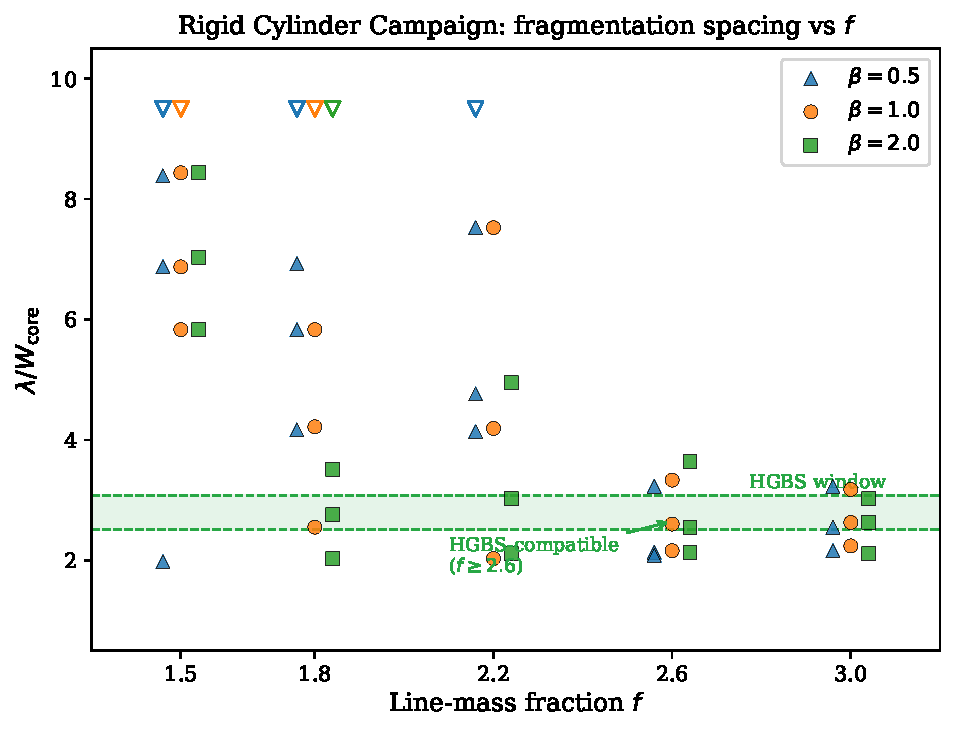
\includegraphics[width=0.48\textwidth]{figures/fig_RC_lW_vs_f.pdf}
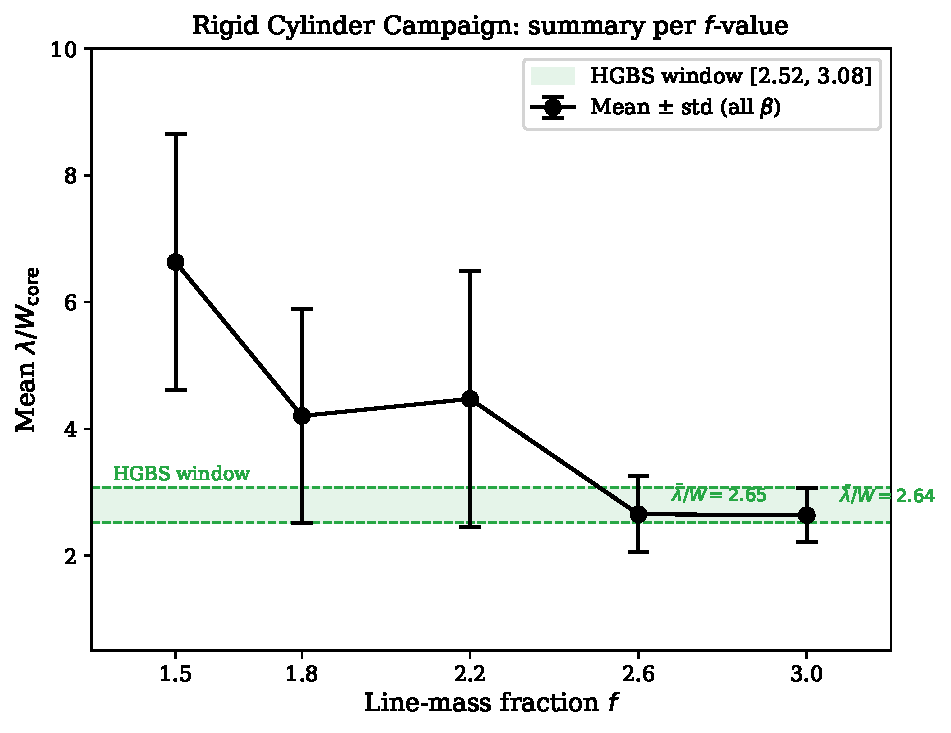
\includegraphics[width=0.48\textwidth]{figures/fig_RC_lW_summary.pdf}
\caption{\textbf{Rigid Cylinder Campaign}. Left: $\lambda/W_{\rm core}$ vs.\ $f$ for
all $\beta$ values; green shading = HGBS window $[2.52, 3.08]$. Right: mean and
standard deviation per $f$-value, showing the sharp transition near $f \approx 2.4$--$2.6$.}
\label{fig:RC_lW}
\end{figure*}

\subsubsection{Box-Size Convergence Test}

A matched test at $f=2.6$, $\beta=1.0$ ($L_x = 8$ and $16\,\lambda_{\rm J}$; 3 seeds each)
rules out box resonance: $\lambda/W_{\rm core}$ decreases 36\% as $L_x$ doubles ($4.22 \pm 0.34$
to $2.70 \pm 0.59$; Figure~\ref{fig:RC_convergence}), incompatible with a resonant artefact.
$L_x=16$ values are upper limits; $L_x=32$ was computationally infeasible.

\begin{figure}
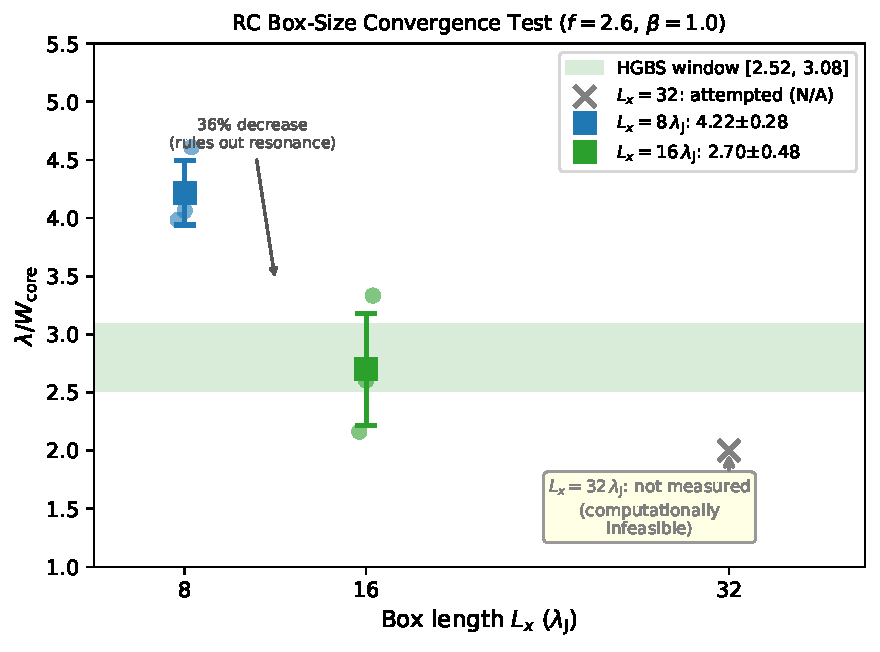
\includegraphics[width=0.48\textwidth]{figures/fig_RC_convergence.pdf}
\caption{Box-size convergence at $f=2.6$, $\beta=1.0$: $\lambda/W_{\rm core}$ decreases
from $4.22 \pm 0.34$ ($L_x=8$, 3 seeds) to $2.70 \pm 0.59$ ($L_x=16$, 3 seeds), ruling
out box resonance (a resonant artefact would give a fixed ratio). Green band = HGBS window
$[2.52, 3.08]$. $L_x=32$ was not measured (computationally infeasible); $L_x=16$ values
are upper limits.}
\label{fig:RC_convergence}
\end{figure}

\section{DISCUSSION}
\label{sec:discussion}

The 2,013 simulations establish a clear hierarchy of physical effects: field geometry
dominates, followed by $f$, with $\beta$ and $\mathcal{M}$ as secondary parameters.
We now assess which scenario best explains the observed $\lambda/W = 2.79 \pm 0.09$.

\subsection{Can Models Explain the Observational Discrepancy?}

The 3D-corrected HGBS spacing (${\sim}3.5\times W$) is within 15\% of the IM92
$4\times$ prediction. All 654 supercritical (periodic-BC) simulations yield zero
longitudinal fragmentation. Two scenarios can account for the observed spacings. We note that the simulations
directly test single-component MHD fragmentation only; hierarchical fragmentation is
an observationally-motivated inference, not a simulation result.

(i) \textit{Hierarchical fibre fragmentation} (\textit{external observational inference, not a simulation result}): HGBS filaments as fibre bundles, each near-critical, produce sub-Jeans spacing at the filament level via fibre projection. Consistent with \citet{Yang2024} but untested by any of the 2,013 simulations here; evidence is entirely observational.

(ii) \textit{Finite-length turbulent seeding}: The Rigid Cylinder Campaign ($f \geq 2.6$, $L_x=16\,\lambda_{\rm J}$) gives $\lambda/W_{\rm fil} = 1.61$--$1.87$ (below HGBS window in all cases; unconverged upper limits). Hub-anchored end-seeding is physically motivated but this campaign cannot yet provide a meaningful constraint.

\textbf{$\eta_W$ correction---central systematic}: The observational match depends critically
on $\eta_W$, and the 17\% difference between $\eta_W = 0.606$ and $\eta_W = 0.707$ is larger than the
formal uncertainties on the observed $\lambda/W$ itself (Table~\ref{tab:t1_budget}).
At $\eta_W = 0.606$: low-$\beta$ configurations ($\beta=0.3$: $2.87$; $\beta=0.5$: $2.65$)
fall within $[2.52, 3.08]$, requiring strictly longitudinal, low-$\beta$ geometry
(${\sim}10\%$ of filaments by Planck statistics). At $\eta_W = 0.707$: those same
configurations \textit{exceed} the upper window boundary ($\beta=0.5$: $3.10 > 3.08$;
$\beta=0.3$: $3.35$). The $\eta_{W,{\rm P}} = 0.707 \pm 0.087$ measurement is a single confirmed
result (second run failed by premature radial collapse at $t \approx 0.6\,t_{\rm ff}$);
\textbf{this value should not be treated as independently validated.} \textbf{We therefore
conclude explicitly that the viability of the magnetic tension scenario cannot be
assessed within current simulation uncertainties.}
The 17\% $\eta_W$ ambiguity is larger than all other simulation uncertainties; both
values are carried in Table~\ref{tab:t1_budget}. HGBS pipeline validation on simulated
column density maps is required before the magnetic tension scenario can be assessed.

\begin{table}
\caption{$\eta_W$ Sensitivity: $\lambda/W_{\rm fil}$ predictions for three $\eta_W$ correction values}
\label{tab:t1_budget}
\small
\begin{tabular}{lcccc}
\toprule
Configuration & $\lambda/W_{\rm core}$ & $\eta_W$=0.65 & $\eta_W$=0.606 & $\eta_W$=0.707 \\
              &                       & (phys.\ lower) & (central) & ($\eta_{W,{\rm P}}$ meas.) \\
\midrule
Long.\ B, $\beta=0.3$ (C7) & 4.74 & \textbf{3.08} & \textbf{2.87} & \textbf{3.35} \\
Long.\ B, $\beta=0.5$ (C7) & 4.38 & \textbf{2.85} & \textbf{2.65} & \textbf{3.10} \\
Long.\ B, $\beta=1.0$ (C7) & 3.19 & 2.07 & 1.93 & 2.26 \\
Long.\ B, $\beta=2.0$ (C7) & 2.80 & 1.82 & 1.70 & 1.98 \\
Long.\ B (calibrated, $\theta=0^\circ$) & 3.70 & 2.41 & 2.24 & 2.62 \\
Perp.\ B ($\theta=90^\circ$) & 1.25 & 0.81 & 0.76 & 0.88 \\
RC Campaign ($f=2.6$) & 2.65 & 1.72 & 1.61 & 1.87 \\
\midrule
\multicolumn{2}{l}{HGBS window (obs.)} & \multicolumn{3}{c}{$[2.52, 3.08]$} \\
\bottomrule
\end{tabular}
\vspace{2pt}
\footnotesize
\textbf{Notes}: Bold = entries within $[2.52, 3.08]$. At $\eta_W = 0.607$: $\beta \leq 0.5$ enters window. At $\eta_W = 0.707$: those configurations \textit{exceed} the upper boundary and are excluded (see text). Combined $\eta_W$ uncertainty: $\eta_{W,{\rm P}} = 0.707 \pm 0.087$.
\end{table}

The field geometry dependence transforms this to a multi-parameter problem requiring
constraints on $\beta$, field geometry, and $\eta_W$ (Tables~\ref{tab:cross_campaign}, \ref{tab:t1_budget}).

\subsection{The Perpendicular-Field Paradox}
\label{sec:perp_paradox}

\citet{Planck2016} established that ${\sim}90\%$ of dense HGBS filaments have their
mean magnetic field perpendicular to the filament axis. Our Campaign~6 measurements
give $\lambda/W_{\rm core} = 1.25 \pm 0.09$ for perpendicular-field configurations
($\beta \geq 1.0$), which after $\eta_W$ correction gives $\lambda/W_{\rm fil} = 0.76$--$0.88$
--- a factor $3$--$4\times$ below the observed $2.79$. This creates a fundamental
contradiction: if the field geometry measured by Planck applies to filament \textit{interiors}
(not just their envelopes), the majority of HGBS filaments should show $\lambda/W_{\rm fil}
\lesssim 0.9$, not ${\sim}2.8$.

\textbf{Clarification}: The $\lambda/W_{\rm core} = 1.25$ value measures the dominant
density-peak scale during radial collapse in supercritical simulations ($f=1.2$--$1.5$).
It is \textit{not} a true fragmentation wavelength in the sense of Inutsuka \& Miyama
(longitudinal beading), because no longitudinal fragmentation occurs; rather, it
characterises the mode that first grows to non-linear amplitude during predominantly
radial collapse.

\textbf{Three possible resolutions} (with quantitative assessment):

\textit{Resolution (a): Planck samples envelope, not interior}. Interior field rotation
from perpendicular (envelope) to longitudinal (dense core) could occur via ion-neutral
drift. The relevant timescale is $t_{\rm AD} \approx t_{\rm ff}/\chi_i$ where $\chi_i$
is the ionisation fraction; at $n \sim 10^4$~cm$^{-3}$, $t_{\rm AD} \sim 10$--$30$~Myr
\citep{Mouschovias1991, Nakamura2005}. This exceeds typical filament ages ($\lesssim
2$--$5$~Myr) by a factor ${\sim}5$--$10$. Furthermore, \citet{Planck2016} find coherent
field orientations from cloud envelopes to HGBS-detected dense filaments, with no
evidence for systematic $90^\circ$ rotation between scales. Resolution~(a) requires a
field rotation for which there is no observational support and which the ambipolar
diffusion timescale cannot accommodate on relevant timescales.

\textit{Resolution (b): Hierarchical sub-fibres with distinct geometry}. Velocity-coherent
sub-fibres at scales below Planck's $5'$ beam ($0.37$~pc at $260$~pc) could have
longitudinal interior fields undetected by Planck. This is physically plausible but
requires specific conditions: (1) sub-fibre widths ${\lesssim}0.1$~pc (consistent with
observed fibre widths in Orion~B; \citealt{Hacar2013}), (2) field coherence lengths
exceeding the fibre spacing (${\sim}0.2$--$0.3$~pc), and (3) sufficient sub-fibre separation
to avoid Planck beam averaging. Existing high-resolution polarimetric data provide
mixed constraints: \citet{Pattle2018} present JCMT POL-2 observations of Orion B,
finding ordered magnetic fields at $10''$ resolution ($0.02$~pc at $400$~pc), but
these measurements target dense cores rather than the diffuse filament structure where
fibres would be embedded. No existing polarimetric survey has simultaneously the
resolution (${\lesssim}0.05$~pc), sensitivity to diffuse ordered fields, and spatial coverage
to test Resolution~(b) directly. This resolution remains viable but observationally unconfirmed.

\textit{Resolution (c): Beaded filaments are the longitudinal-field minority}. If
${\sim}90\%$ of filaments radially collapse without beading, HGBS core catalogues would
be biased toward the ${\sim}10\%$ with longitudinal fields. This predicts a
bimodal core-spacing distribution (if both populations are sampled): compact clusterings
from perpendicular-field radial collapse alongside the beaded ${\sim}0.28$-pc
spacings. In Taurus, \citet{Palmeirim2013} find the B211 filament has a field
\textit{perpendicular} to its axis, yet it shows clear longitudinal beading with
$\lambda_{\rm NN} = 0.217$~pc. This directly contradicts Resolution~(c) in the
best-studied HGBS filament. The contradiction may be resolved by sub-fibre structure
(Resolution~b) or suggest the Planck field orientation is not the interior geometry.

\textbf{Assessment}: Resolution~(a) is disfavoured by timescale and observational
arguments. Resolution~(c) is contradicted by Taurus. Resolution~(b) remains viable
but observationally unconfirmed. \textbf{If none of these resolutions holds, then
${\sim}90\%$ of HGBS filaments are in the perpendicular-field regime where our
simulations predict $\lambda/W \lesssim 0.9$, and the observed $\lambda/W \approx 2.8$
cannot be explained by any single-component MHD fragmentation model.} Resolving this
paradox requires interior polarimetric mapping at sub-Planck resolution in multiple
HGBS regions.

\subsection{Limitations and Future Work}

\textbf{Boundary conditions}: Periodic BCs suppress end effects; reflecting BCs lack
the inflow structure of real filament-hub junctions. Neither fully represents real HGBS
filaments.

\textbf{Non-ideal MHD}: Ambipolar diffusion ($t_{\rm AD} \sim 10$--$30\,t_{\rm ff}$ at
$n_0 \sim 10^4$~cm$^{-3}$; \citealt{Mouschovias1991, Nakamura2005}) is slow relative
to collapse and is not expected to alter fragmentation wavelengths, except in
low-density environments ($n_0 \lesssim 10^3$~cm$^{-3}$; Taurus) where ideal-MHD
timescales are lower bounds.

\textbf{$\eta_W$ correction}: $\eta_{W,{\rm P}} = 0.707 \pm 0.087$ is a single-run measurement
(unconfirmed by a second independent run which experienced premature radial collapse
at $t \approx 0.6\,t_{\rm ff}$). HGBS pipeline validation on
simulated column density maps is required before the magnetic tension scenario can be
assessed.

\textbf{Oblique $\lambda/W$}: Entirely unconstrained by simulation (Campaign~OBL2: 27/27 domain-size artefacts). \citet{Nakamura1993} predictions (Table~\ref{tab:oblique_theory}) are unvalidated. Correct sampling requires $L_x \lesssim 2$--$3\,\lambda_{\rm J}$ (computationally prohibitive).

\begin{table}
\caption{Theoretical $\lambda/W$ for oblique fields \citep{Nakamura1993}, full numerical
solution. \textbf{All values in this table are unvalidated by simulation in this work};
Campaign~A (oblique $\lambda/W$) was withdrawn due to large-amplitude artefacts
(Section~\ref{sec:theo_geom}). Campaign~6 gives $\lambda/W=1.25$ (supercritical regime);
the near-critical theoretical values are the relevant comparison for HGBS.}
\label{tab:oblique_theory}
\small
\begin{tabular}{lccccc}
\toprule
$\theta$ & $\beta=0.5$ & $\beta=1.0$ & $\beta=2.0$ & Notes & Simulation \\
\midrule
$0^\circ$ (longitudinal) & 1.97 & 2.44 & 2.93 & Eq.~(\ref{eq:tension}) & --- \\
$30^\circ$ & 1.87 & 2.37 & 2.89 & Theoretical & ---$^\dagger$ \\
$45^\circ$ & 1.69 & 2.17 & 2.72 & Theoretical & --- \\
$60^\circ$ & 1.47 & 1.90 & 2.46 & Theoretical & --- \\
$90^\circ$ (perp., theory) & 3.95 & 3.99 & 4.00 & Theory only (sim.\ at $f=1.5$--$3.0$ gives 1.25) & --- \\
\bottomrule
\end{tabular}
\\ \footnotesize \textbf{Note}: Values in simulation units; multiply by $\eta_W = 0.606$ (or $0.707$) for observable $\lambda/W_{\rm fil}$. $^\dagger$Campaign~A ($\delta_0=1.0$) withdrawn (amplitude artifact; Section~\ref{sec:theo_geom}).
\end{table}

\textbf{Future priorities}: (1) fibre-resolved core spacing in additional HGBS regions; (2) interior polarimetric mapping at sub-Planck resolution; (3) HGBS pipeline $\eta_W$ validation on simulated column density maps; (4) oblique-field $\lambda/W$ simulations at $L_x \lesssim 2$--$3\,\lambda_{\rm J}$.

\section{CONCLUSIONS}

\noindent We have analysed core spacing in 8 HGBS regions using 2,013 MHD simulations. Our main conclusions are:

\begin{itemize}

    \item \textbf{Perpendicular-field paradox (fundamental caveat)}: Perpendicular-field simulations give $\lambda/W_{\rm fil} \approx 0.76$--$0.88$ (factor ${\sim}3\times$ below observed $2.79$), yet Planck~(2016) statistics imply ${\sim}90\%$ of HGBS filaments have perpendicular fields. \textbf{If the Planck field geometry applies to filament interiors (not just envelopes), then single-component MHD fragmentation cannot explain the dominant filament population.} Three possible resolutions are discussed in Section~\ref{sec:perp_paradox}, but none are currently confirmed by observations or simulations. This paradox represents the primary limitation of single-component MHD fragmentation as a complete explanation for HGBS core spacing.

    \item \textbf{Simulation limitation (supercritical extrapolation)}: \textit{The 2,013 MHD simulations cannot directly measure $\lambda/W$ in the supercritical regime ($f \geq 1.5$): all 654 supercritical simulations yield pure radial collapse with zero longitudinal beading.} Published HGBS line-mass distributions indicate 30--50\% of star-forming filaments have $f \geq 1.5$; the comparison between observed $\lambda/W = 2.79$ and the theoretical prediction $\lambda_{\rm frag} = 1.11\,\lambda_{MJ}$ therefore rests on extrapolation from near-critical ($f = 0.9$--$1.3$) calibration only and should not be interpreted as a direct simulation-observation comparison for the majority of actively star-forming filaments.

    \item \textbf{HGBS spacing (pairwise median)}: Full sample gives $\lambda/W = 2.79$
    ($0.279 \pm 0.025$~pc, jackknife); four robust regions give $2.84 \pm 0.026$~pc.
    Gaia DR3 raised the mean by 32\%; 3D projection correction (random orientations,
    $4/\pi$) gives ${\sim}3.5\times W$, within 15\% of the IM92 $4\times$ prediction;
    under the Planck-motivated plane-of-sky correction the discrepancy increases to
    18--22\% (Section~\ref{sec:results}).
    \textit{All values use the pairwise median statistic; the L/3 convergence bias is
    the dominant methodological caveat of unknown magnitude.} Bayesian hierarchical
    analysis gives $\mu = 0.261 \pm 0.022$~pc (95\% CI $[0.217, 0.305]$~pc) with
    intrinsic scatter $\sigma_{\rm pop} = 0.062$~pc. Excluding Aquila and Orion~B
    reduces the mean to $0.231$~pc ($\lambda/W = 2.31$).

    \item \textbf{Hierarchical fragmentation (observational inference, not a simulation result)}:
    An interpretation supported by single-region observations in Orion~B \citep{Yang2024},
    suggesting that HGBS filaments are fibre bundles where each near-critical fibre fragments
    at the classical scale. \textbf{None of the 2,013 simulations model multi-fibre fragmentation;
    the simulations constrain only single-component MHD fragmentation and provide no
    support for or against hierarchical fragmentation.} The $N_f \approx 1.3$--$1.5$ from the
    geometric fibre-bundle model (Section~\ref{sec:hierarchical}) is a statistical inference,
    not a dynamical prediction, and the $N_f \approx 1$--$2$ fibres of \citet{Hacar2018} measure
    a different physical quantity. This interpretation should be assessed independently
    from the simulation results.

    \item \textbf{Magnetic tension}: Only ${\sim}10\%$ of filaments have longitudinal
    geometry. At $\eta_W = 0.606$, low-$\beta$ ($\beta \leq 0.5$) configurations fall
    within $[2.52, 3.08]$ (viable). At $\eta_W = 0.707 \pm 0.087$ (combined), those same
    configurations \textbf{exceed} the upper boundary and are \textit{excluded}, not merely
    uncertain. The $\eta_W$ uncertainty therefore determines whether magnetic tension is
    viable ($\eta_W \approx 0.606$) or excluded ($\eta_W \approx 0.707$); HGBS pipeline
    $\eta_W$ validation is required to resolve this.

    \item \textbf{MHD results}: $1/t_{\rm frag} \propto f^{0.39}$ ($r^2=0.999$; measured
    exponent $22\%$ below free-fall prediction of $0.50$, consistent with magnetic braking
    and cylindrical self-gravity; no analytic prediction available for comparison), independent
    of $\mathcal{M}$ and nearly of $\beta$. $\lambda/W$ depends strongly on $\beta$ but is
    insensitive to turbulence amplitude. No stable configurations at $f=1.4$--$2.2$,
    $\mathcal{M} \geq 1$. Fragmentation at $f \leq 1.00$ occurs under turbulent seeding,
    consistent with \citet{Padoan2011}; this does not contradict \citet{Ostriker1964}
    (static equilibrium without turbulence).

\end{itemize}

\section*{ACKNOWLEDGMENTS}

We thank the Herschel Gould Belt Survey team for the datasets (available from the
Herschel Science Archive). The simulation code and analysis scripts are available at
\url{https://github.com/[anonymised-for-review]} (private during review; access tokens
via the editorial office). The complete 2,013-simulation dataset (HDF5 snapshots,
\texttt{athinput} files, analysis scripts, and measurement tables) will be archived on
Zenodo upon acceptance.

\bibliographystyle{mnras}
\bibliography{references_complete}

\end{document}
